%! Author = crist
%! Date = 24/10/2026

\spacing{1.3}
%----------------------------------------------------------------------------------------
%	UNIDAD 2: EL ÁTOMO Y LA TABLA PERIÓDICA (4.º ESO)
%   Figuras: images/UD2/*.pdf (fuente HTML en images/UD2/html, SVG en images/UD2/svg)
%----------------------------------------------------------------------------------------

%------------------------------------------------
% Comandos propios de la unidad
%------------------------------------------------
% Configuración electrónica en letra recta: \conf{1s^2~2s^2~2p^6}
\providecommand{\conf}[1]{\(\mathrm{#1}\)}

% Espectros dibujados con TikZ (para los ejercicios)
\pgfdeclarehorizontalshading{arcoiris}{100bp}{%
    rgb(0bp)=(0.45,0,0.55); rgb(18bp)=(0.25,0,1); rgb(32bp)=(0,0.55,1); rgb(42bp)=(0,0.9,0.9);
    rgb(52bp)=(0,0.9,0.2); rgb(65bp)=(1,1,0); rgb(78bp)=(1,0.5,0); rgb(90bp)=(1,0,0); rgb(100bp)=(0.45,0,0)}
% Posiciones de las rayas entre 0 y 1 (0 = violeta, 1 = rojo)
\providecommand{\espectrocontinuo}{%
    
\begin{tikzpicture}[x=6cm,y=0.7cm]
        \shade[shading=arcoiris] (0,0) rectangle (1,1);
    \end{tikzpicture}}
\providecommand{\espectroemision}[1]{%
    \begin{tikzpicture}[x=6cm,y=0.7cm]
        \fill[black] (0,0) rectangle (1,1);
        \foreach \p/\c in {#1} {\fill[\c] (\p-0.005,0) rectangle (\p+0.005,1);}
    \end{tikzpicture}}
\providecommand{\espectroabsorcion}[1]{%
    \begin{tikzpicture}[x=6cm,y=0.7cm]
        \shade[shading=arcoiris] (0,0) rectangle (1,1);
        \foreach \p in {#1} {\fill[black] (\p-0.005,0) rectangle (\p+0.005,1);}
    \end{tikzpicture}}

% Mapa conceptual del tema (fuente en images/mapas_conceptuales/html/temas.js)
\begin{figure}[H]
    \centering
    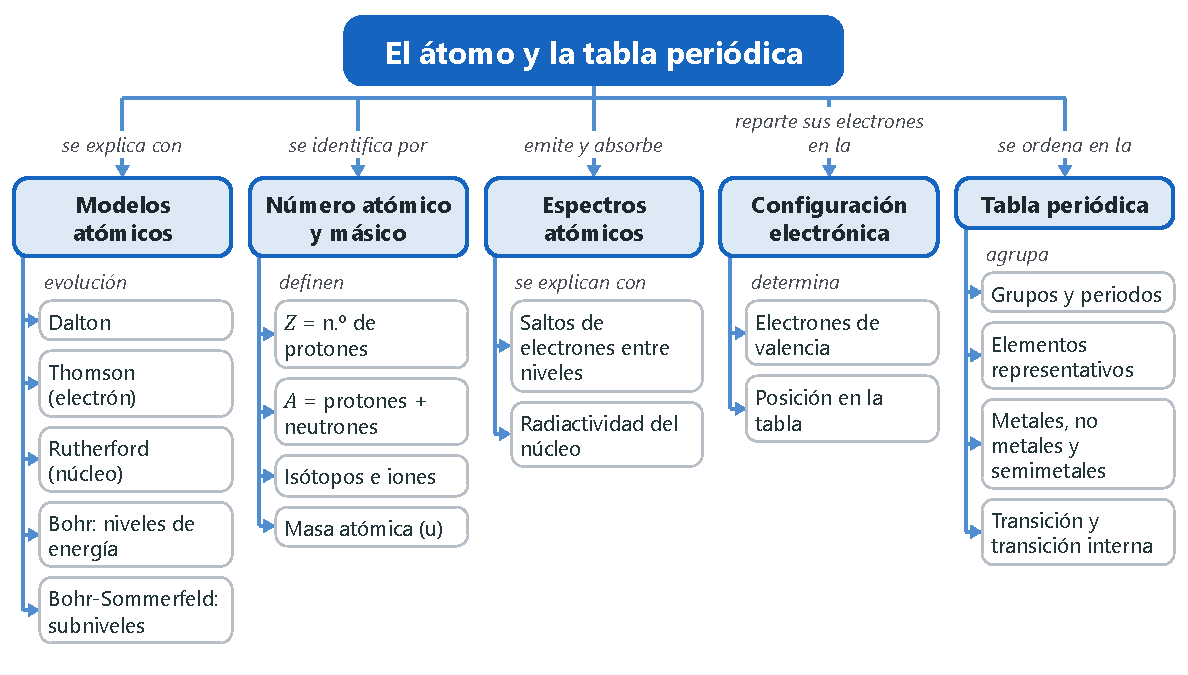
\includegraphics[width=\textwidth]{images/mapas_conceptuales/mapa_UD2}
\end{figure}

%========================================================================================
%\section*{Para empezar: las tierras raras}
%\addcontentsline{toc}{section}{Para empezar: las tierras raras}
%========================================================================================
%
%Con el nombre de \textbf{tierras raras} se conoce a un grupo de \textbf{17 elementos químicos}: los 15 lantanoides, más el escandio y el itrio. Estos dos últimos se incluyen en el grupo porque aparecen en los mismos yacimientos y tienen propiedades químicas, ópticas y magnéticas muy parecidas.
%
%Aunque su nombre sugiere lo contrario, no son tan escasos; lo difícil es encontrarlos concentrados y separarlos unos de otros. Hoy son imprescindibles en telecomunicaciones, electrónica, medicina, nanotecnología, electrodomésticos o en la producción y almacenamiento de energía. Sin ellos no existirían los vehículos eléctricos, los aerogeneradores ni muchas placas solares: nuestra tecnología retrocedería varias décadas.
%
%Un teléfono móvil contiene entre 65 y 70 elementos distintos, y ocho de ellos son tierras raras: gracias a ellos la pantalla tiene colores intensos, los altavoces suenan y el teléfono vibra. En medicina se emplean en resonancias magnéticas, equipos de rayos X, tomografías y en algunas terapias contra el cáncer.
%
%\begin{remark}
%    \textbf{Tierras raras y Objetivos de Desarrollo Sostenible.} Su uso en diagnóstico y tratamiento médico las relaciona con el \textbf{ODS 3} (\emph{Salud y bienestar}); su papel en las «tecnologías limpias» (baterías, aerogeneradores, placas solares) las conecta con el \textbf{ODS 7} (\emph{Energía asequible y no contaminante}). Sin embargo, se extraen en minas a cielo abierto con un elevado coste ambiental.
%\end{remark}
%
%\begin{exercise}
%    Busca en la tabla periódica el nombre, el símbolo y el número atómico de las 17 tierras raras.
%    \begin{solu}
%        Escandio, Sc, 21; itrio, Y, 39; lantano, La, 57; cerio, Ce, 58; praseodimio, Pr, 59; neodimio, Nd, 60; prometio, Pm, 61; samario, Sm, 62; europio, Eu, 63; gadolinio, Gd, 64; terbio, Tb, 65; disprosio, Dy, 66; holmio, Ho, 67; erbio, Er, 68; tulio, Tm, 69; iterbio, Yb, 70; lutecio, Lu, 71.
%    \end{solu}
%\end{exercise}
%
%\begin{exercise}
%    ¿Están todas las tierras raras en el mismo grupo y en el mismo período de la tabla?
%    \begin{solu}
%        No. Los lantanoides están todos en el período 6 (en la fila separada de la parte inferior). El escandio y el itrio están en el mismo grupo (grupo 3), pero en períodos distintos (4 y 5, respectivamente).
%    \end{solu}
%\end{exercise}
%
%\begin{exercise}
%    Explica con tus palabras por qué se afirma que, sin estos elementos, la tecnología retrocedería varias décadas. ¿En qué sectores se usan y qué aplicaciones tienen?
%    \begin{solu}
%        Porque forman parte de casi todos los dispositivos electrónicos y de las tecnologías energéticas actuales: sin ellos no habría transición energética ni tecnología punta. Se usan en telecomunicaciones, electrónica (móviles, ordenadores, tabletas), medicina, energía, electrodomésticos y nanotecnología.
%    \end{solu}
%\end{exercise}
%
%\begin{exercise}
%    Teniendo en cuenta lo que has leído, ¿por qué es tan importante reciclar los móviles y otros aparatos electrónicos? Relaciona tu respuesta con los ODS 3 y 7.
%    \begin{solu}
%        Porque contienen elementos valiosos y difíciles de obtener, cuya extracción tiene un alto coste ambiental. Reciclarlos permite recuperarlos sin abrir nuevas minas. Estos elementos se usan en el diagnóstico y tratamiento de enfermedades (ODS 3) y en las tecnologías limpias de producción de energía (ODS 7).
%    \end{solu}
%\end{exercise}

%========================================================================================
\section{Los primeros modelos atómicos y la radiactividad}
%========================================================================================

Hace unos 2\,400 años, los filósofos griegos \textbf{Leucipo} y \textbf{Demócrito} propusieron que la materia no puede dividirse indefinidamente: tiene que existir una porción mínima e indivisible, a la que llamaron \textbf{átomo}, palabra que significa «\emph{que no se puede dividir}». Era una idea filosófica, sin experimentos que la apoyasen.

\begin{definition}[Modelo científico]
    Un \textbf{modelo} es una representación simplificada de la realidad que intenta explicar los hechos experimentales.
    Es mejor cuantos más hechos explica. Si aparece un descubrimiento que el modelo no puede explicar, el modelo se revisa o se sustituye por otro.
\end{definition}

\begin{figure}[H]
    \centering
    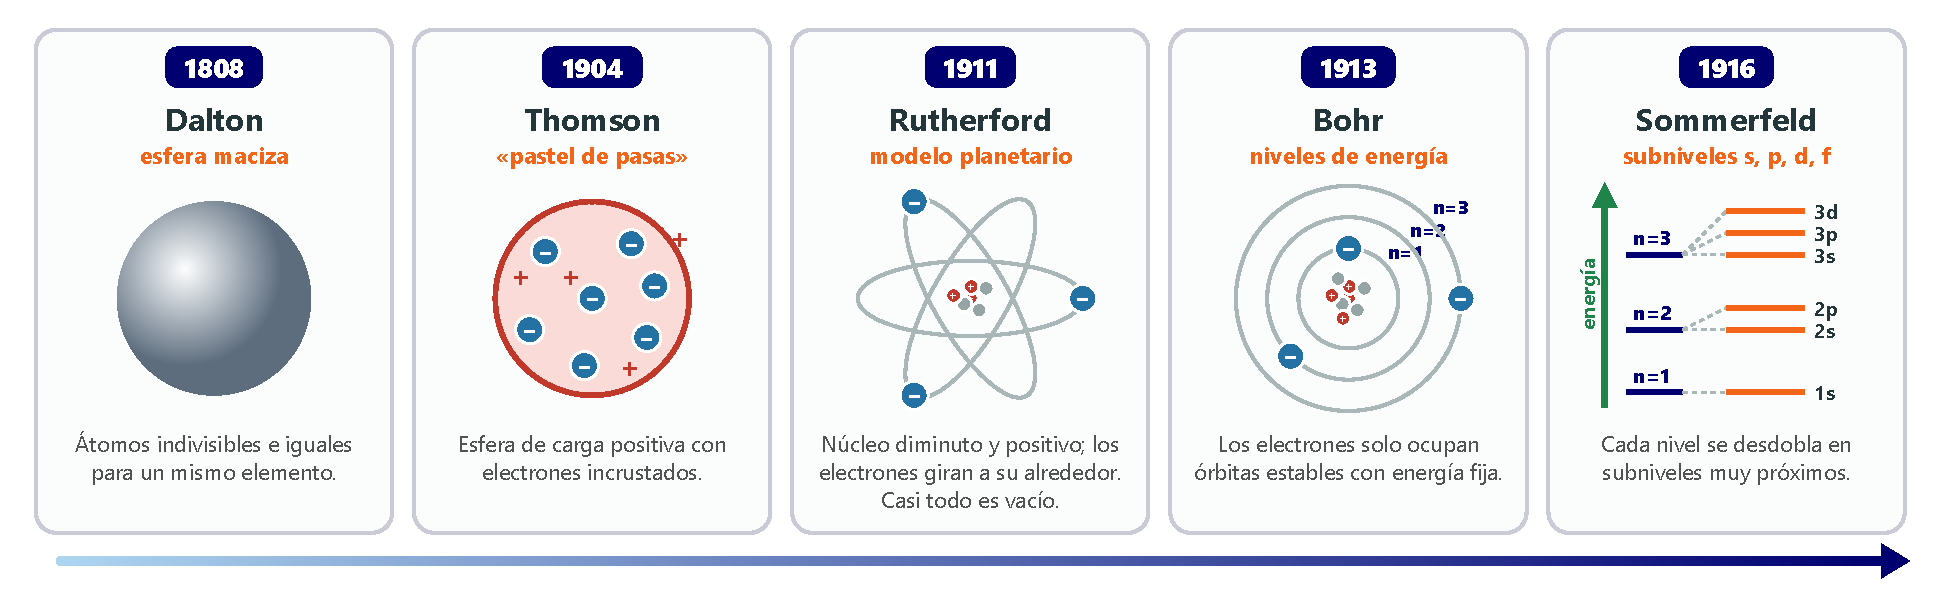
\includegraphics[width=\textwidth]{images/UD2/modelos_atomicos}
    \caption{Evolución de los modelos atómicos que estudiarás en esta unidad.}
    \label{fig:modelos_atomicos}
\end{figure}

\subsection{La teoría atómica de Dalton}

En 1808, el químico inglés \textbf{John Dalton} recuperó la idea de átomo, pero esta vez para explicar resultados experimentales (las leyes de las reacciones químicas). Su \textbf{teoría atómica} se resume en estos postulados:

\begin{enumerate}[label=\numberballblue]
    \item La materia está formada por partículas diminutas, \textbf{indivisibles e inalterables}, llamadas átomos.
    \item Todos los átomos de un mismo elemento son \textbf{iguales} entre sí: tienen la misma masa y las mismas propiedades.
    \item Los átomos de elementos distintos tienen masas y propiedades \textbf{diferentes}.
    \item Los compuestos se forman al unirse átomos de dos o más elementos en una \textbf{proporción de números enteros sencillos}.
\end{enumerate}

\subsection{El átomo es divisible: el electrón y el protón}

El modelo de Dalton fue aceptado durante buena parte del siglo \textsc{xix}. Sin embargo, a finales de ese siglo, los experimentos con \textbf{tubos de descarga} (tubos de vidrio con un gas a muy baja presión sometido a un voltaje muy alto) demostraron que los átomos contienen partículas más pequeñas.

\begin{itemize}
    \item \negsubro{El electrón.} En 1897, \textbf{J.\,J. Thomson} demostró que los \emph{rayos catódicos} que se producen en el tubo son haces de partículas con carga negativa, que salen del electrodo negativo (cátodo) y se dirigen al positivo (ánodo). Stoney las había llamado \textbf{electrones}.
    \item \negsubro{El protón.} En 1886, \textbf{E. Goldstein}, usando un cátodo perforado, observó unos rayos positivos (\emph{rayos canales}) que viajan en sentido contrario, del ánodo al cátodo. La partícula positiva más ligera se obtiene con hidrógeno; Rutherford la llamó \textbf{protón} en 1925.
\end{itemize}

\begin{figure}[H]
    \centering
    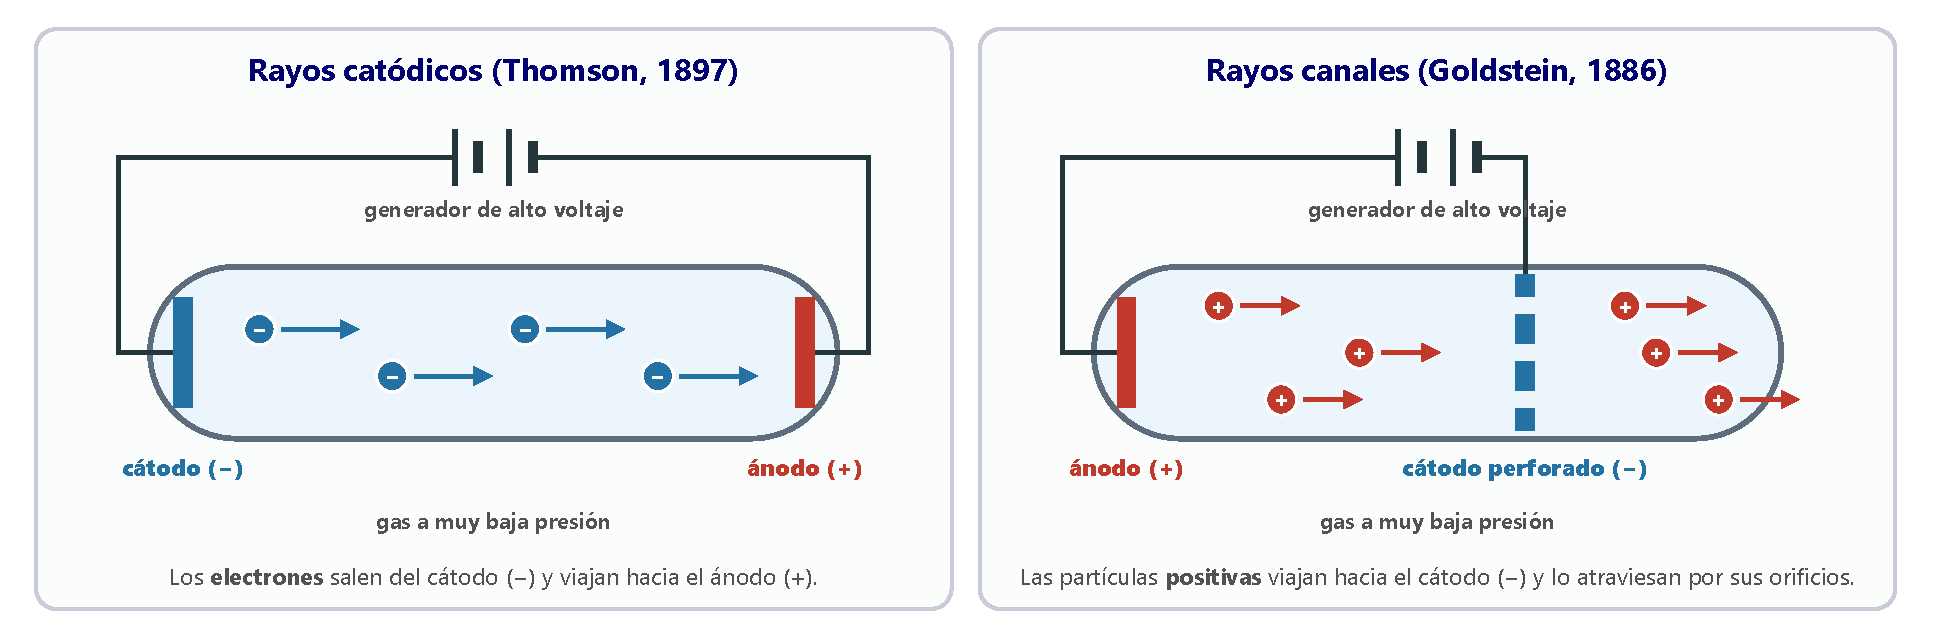
\includegraphics[width=\textwidth]{images/UD2/tubos_descarga}
    \caption{Tubos de descarga: descubrimiento del electrón (izquierda) y del protón (derecha).}
    \label{fig:tubos_descarga}
\end{figure}

\begin{table}[H]
    \centering
    % --- tabla antigua ---
    % \begin{tblr}{colspec={lccc}, hlines, vlines, row{1}={bg=ocre!85, fg=white, font=\bfseries}, column{1}={bg=ocre!15, font=\bfseries}, cell{1}{1}={bg=ocre!85, fg=white}}
        % Partícula & Electrón & Protón & Neutrón \\
        % Carga eléctrica & \qty{-1.602e-19}{\coulomb} & \qty{+1.602e-19}{\coulomb} & sin carga \\
        % Masa & \qty{9.109e-31}{\kg} & \qty{1.673e-27}{\kg} & \qty{1.675e-27}{\kg} \\
        % Descubrimiento & Thomson, 1897 & Goldstein, 1886 & Chadwick, 1932 \\
    % \end{tblr}
    % --- tabla nueva ---
    \begin{tabular}{@{}lccc@{}}
        \toprule
        \textbf{Partícula} & \textbf{Electrón} & \textbf{Protón} & \textbf{Neutrón} \\
        \midrule
        \textbf{Carga eléctrica} & \qty{-1.602e-19}{\coulomb} & \qty{+1.602e-19}{\coulomb} & sin carga \\[3pt]
        \textbf{Masa} & \qty{9.109e-31}{\kg} & \qty{1.673e-27}{\kg} & \qty{1.675e-27}{\kg} \\[3pt]
        \textbf{Descubrimiento} & Thomson, 1897 & Goldstein, 1886 & Chadwick, 1932 \\
        \bottomrule
    \end{tabular}
    \caption{Características de las partículas subatómicas.}
    \label{tab:particulas}
\end{table}

\begin{remark}
    El protón y el electrón tienen cargas \textbf{iguales en valor y de signo contrario}, pero el protón es unas \textbf{1\,836 veces más pesado} que el electrón. El neutrón (que estudiarás más adelante) tiene una masa casi igual a la del protón.
\end{remark}

¿Qué conclusiones se obtienen de estos descubrimientos?
\begin{enumerate}[label=\numberballgreen]
    \item El átomo \textbf{sí es divisible}: contiene partículas subatómicas.
    \item Los electrones tienen \textbf{carga negativa}.
    \item El resto del átomo tiene \textbf{carga positiva} y contiene casi toda la masa.
    \item Como el átomo es eléctricamente neutro, el número de cargas negativas (electrones) es \textbf{igual} al de cargas positivas (protones).
\end{enumerate}

\begin{exercise}
    La carga de un electrón es \qty{-1.6e-19}{\coulomb}. ¿Cuántos electrones hacen falta para reunir una carga total de \qty{-2}{\coulomb}?
    \begin{solu}
        \textcolor{blue}{Dividimos la carga total entre la carga de un electrón:}
        \[ N = \frac{Q}{q_e} = \frac{\qty{-2}{\coulomb}}{\qty{-1.6e-19}{\coulomb}} = \textcolor{red}{\num{1.25e19}\ \text{electrones}} \]
    \end{solu}
\end{exercise}

\begin{exercise}
    ¿Podía explicar la teoría de Dalton la existencia de electrones y protones? Razónalo.
    \begin{solu}
        No. Para Dalton el átomo era indivisible, es decir, no tenía partes. La existencia de partículas más pequeñas que el átomo contradice directamente su primer postulado.
    \end{solu}
\end{exercise}

\subsection{El modelo atómico de Thomson}

Con estos datos, Thomson propuso en 1904 el primer modelo de átomo con partes, conocido como modelo del \textbf{«pastel de pasas»}: el átomo sería una \textbf{esfera de carga positiva} en la que los \textbf{electrones} están incrustados, como las pasas en un bizcocho. La carga positiva total compensa la negativa, de modo que el átomo es neutro (figura~\ref{fig:modelo_thomson}).

\begin{figure}[H]
    \centering
    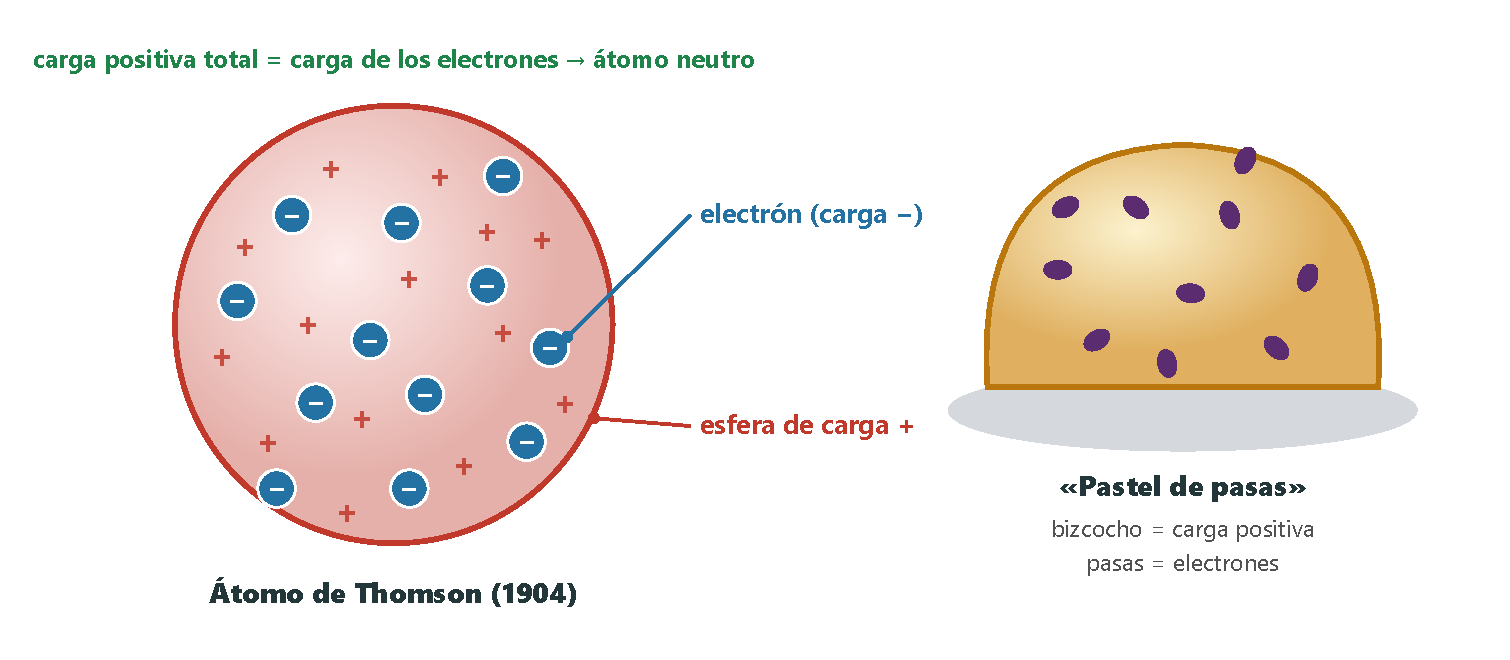
\includegraphics[width=0.9\textwidth]{images/UD2/modelo_thomson}
    \caption{Modelo atómico de Thomson: los electrones están incrustados en una esfera de carga positiva, como las pasas en un bizcocho.}
    \label{fig:modelo_thomson}
\end{figure}

Este modelo se aceptó hasta que nuevos experimentos demostraron que el interior del átomo no podía ser así.

\subsection{El modelo planetario de Rutherford}

\paragraph{El átomo no es un pastel de pasas.} En 1911, \textbf{Ernest Rutherford} y sus colaboradores \textbf{Geiger} y \textbf{Marsden} bombardearon una lámina de oro muy fina con \textbf{partículas alfa} (partículas positivas y rápidas). Una pantalla de sulfuro de zinc colocada alrededor emitía un destello cada vez que recibía una partícula. Observaron que:

\begin{itemize}
    \item La \textbf{inmensa mayoría} de las partículas \textbf{atravesaba} la lámina sin desviarse.
    \item \textbf{Algunas} se \textbf{desviaban} bastante de su trayectoria.
    \item \textbf{Muy pocas} (aproximadamente una de cada 10\,000) \textbf{rebotaban} y volvían hacia la fuente.
\end{itemize}

\begin{figure}[H]
    \centering
    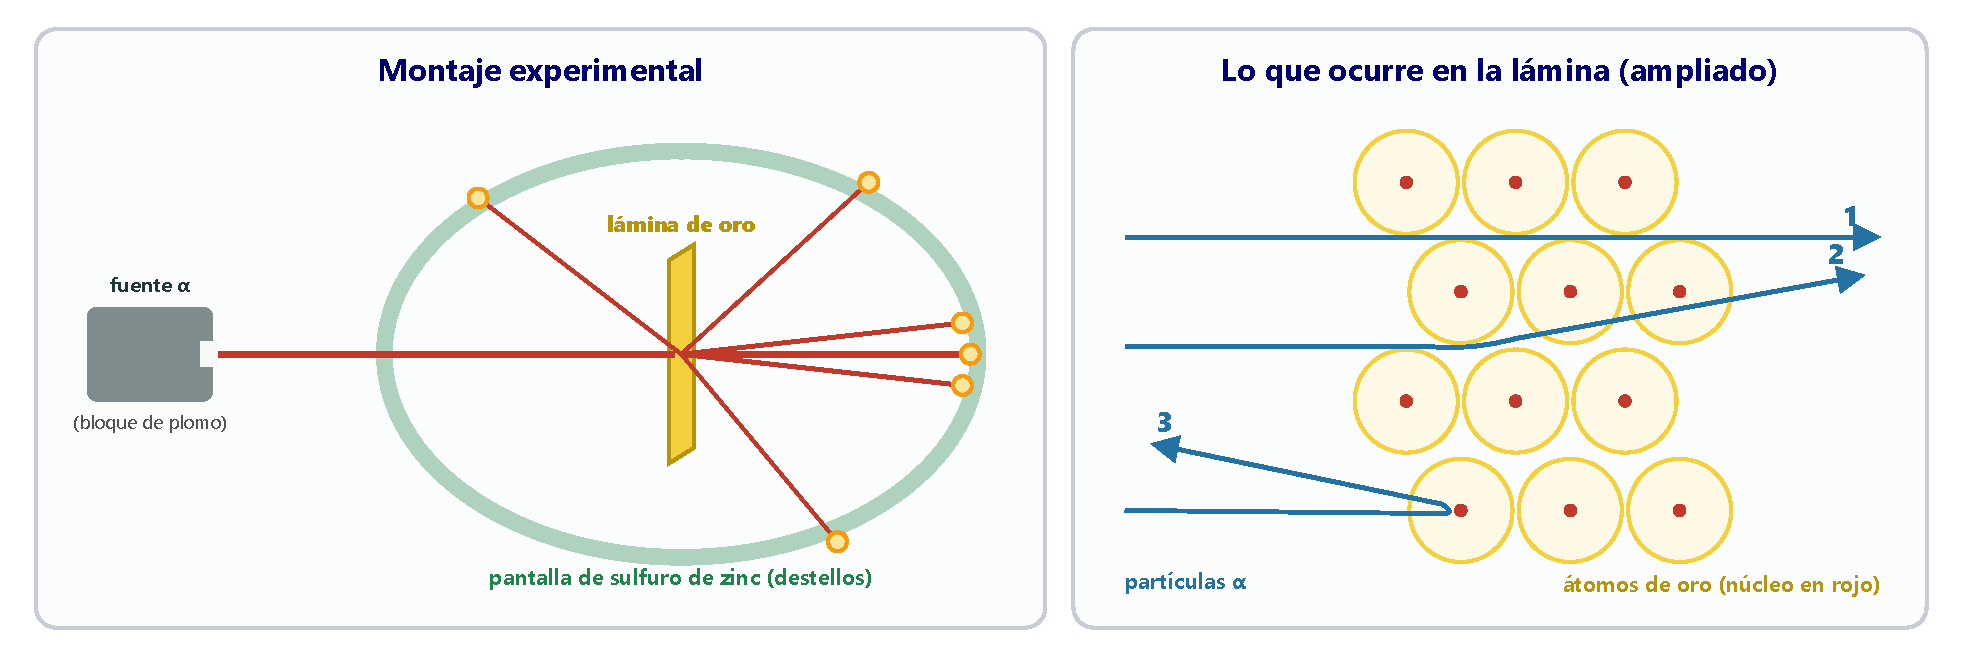
\includegraphics[width=\textwidth]{images/UD2/experimento_rutherford}
    \caption{Experimento de Rutherford, Geiger y Marsden. A la derecha: (1) la partícula pasa lejos de los núcleos y no se desvía; (2) pasa cerca de un núcleo y es repelida; (3) choca de frente con un núcleo y rebota.}
    \label{fig:experimento_rutherford}
\end{figure}

El modelo de Thomson no podía explicar el rebote de algunas partículas: en una esfera positiva «blanda» y uniforme no hay nada lo bastante concentrado para hacerlas volver.

\paragraph{El modelo planetario.} Rutherford propuso entonces un modelo nuevo:
\begin{itemize}
    \item El átomo es, en su mayor parte, \textbf{espacio vacío}.
    \item En el centro hay un \textbf{núcleo} diminuto en el que se concentran \textbf{toda la carga positiva} y \textbf{casi toda la masa} del átomo.
    \item Los \textbf{electrones} giran a gran velocidad alrededor del núcleo, a una distancia muy grande comparada con su tamaño, como los planetas alrededor del Sol. Esta zona se llama \textbf{corteza}.
\end{itemize}

Así se explica el experimento: casi todas las partículas atraviesan el espacio vacío (1); las que pasan cerca de un núcleo son repelidas porque ambos son positivos (2); y las pocas que chocan de frente contra un núcleo rebotan (3).

\paragraph{El descubrimiento del neutrón.} Los protones no bastaban para explicar la masa de los núcleos: el núcleo de helio, por ejemplo, tiene dos protones pero una masa cuatro veces la del hidrógeno. Rutherford supuso que debía existir otra partícula en el núcleo, con masa pero sin carga. En 1932, \textbf{James Chadwick} la descubrió y la llamó \textbf{neutrón}.

\begin{remark}
    \textbf{¡Qué vacío está el átomo!} Si el núcleo de un átomo tuviera el tamaño de una canica colocada en el centro de un campo de fútbol, los electrones estarían girando más allá de las gradas.
\end{remark}

\paragraph{Electrización de la materia y formación de iones.} El modelo de Rutherford explica fenómenos como la electrización. Un cuerpo neutro tiene tantas cargas positivas como negativas. Al frotarlo, puede \textbf{ganar} electrones (y se carga negativamente) o \textbf{perder} electrones (y se carga positivamente). Los protones nunca se mueven: están fijos en el núcleo.

Del mismo modo, un átomo neutro puede ganar o perder electrones y convertirse en un \textbf{ion}:
\begin{itemize}
    \item Si \textbf{pierde} electrones queda con carga positiva: es un \textbf{catión} (por ejemplo, \ch{Na+}).
    \item Si \textbf{gana} electrones queda con carga negativa: es un \textbf{anión} (por ejemplo, \ch{Cl-}).
\end{itemize}

\begin{figure}[H]
    \centering
    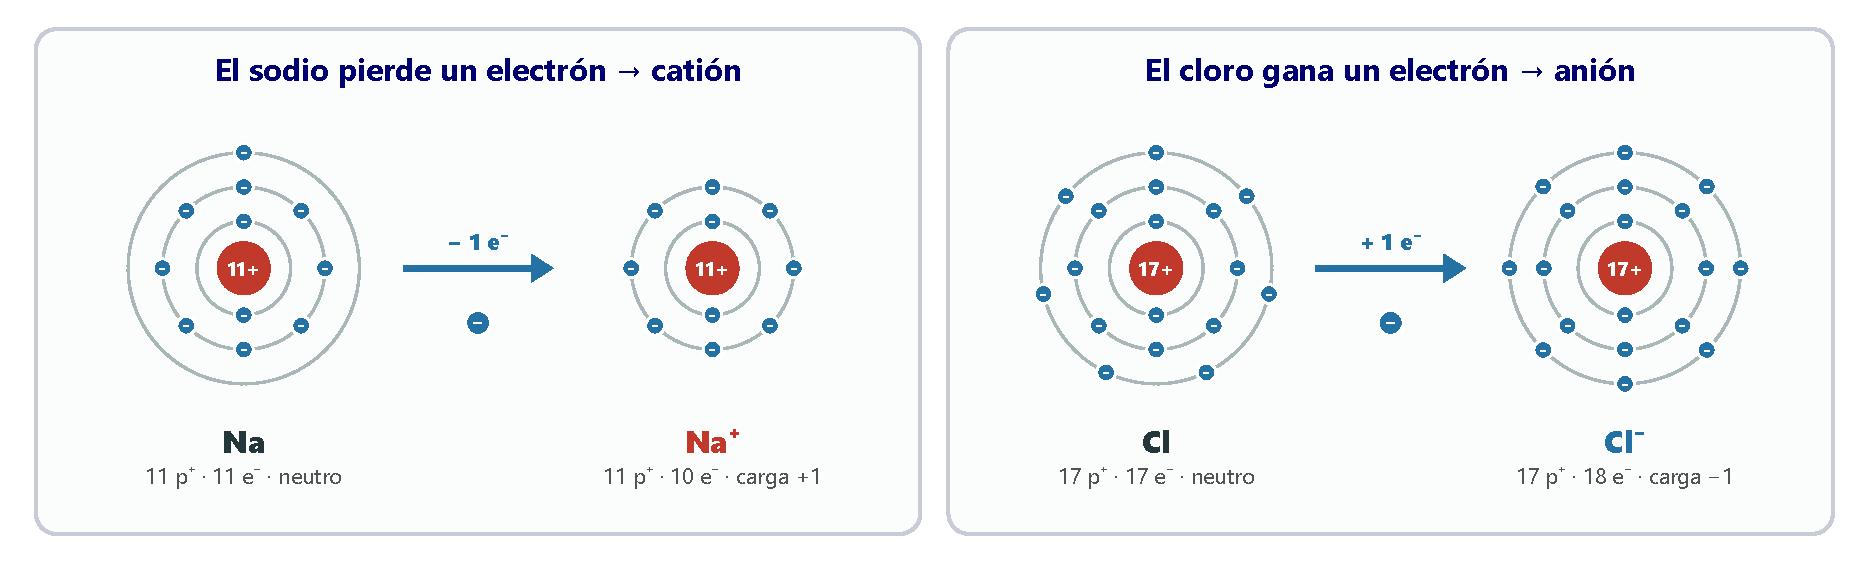
\includegraphics[width=\textwidth]{images/UD2/iones}
    \caption{Formación de un catión y de un anión: solo cambia el número de electrones.}
    \label{fig:iones}
\end{figure}

\subsection{Un fenómeno nuclear: la radiactividad}

En 1896, \textbf{Henri Becquerel} descubrió por casualidad que unas placas fotográficas envueltas en papel se habían velado al guardarlas junto a un mineral de uranio. El mineral emitía algo capaz de atravesar el papel. Marie y Pierre Curie estudiaron el fenómeno, que llamaron \textbf{radiactividad}.

\begin{definition}[Radiactividad]
    Es el fenómeno por el cual los \textbf{núcleos} de algunos átomos emiten \textbf{espontáneamente} partículas y radiaciones, transformándose en núcleos de otros elementos.
\end{definition}

Rutherford comprobó que, al hacer pasar estas emisiones entre dos placas cargadas, se separaban en tres tipos:

\begin{itemize}
    \item \negsubro{Partículas alfa (\(\alpha\)).} Formadas por \textbf{dos protones y dos neutrones} (son núcleos de helio). Tienen carga positiva, por lo que se desvían hacia la placa negativa. Son relativamente lentas y muy poco penetrantes: \textbf{una hoja de papel las detiene}.
    \item \negsubro{Partículas beta (\(\beta\)).} Son \textbf{electrones} muy rápidos. Se desvían mucho hacia la placa positiva y son más penetrantes: atraviesan el papel, pero \textbf{una lámina de aluminio de unos milímetros las detiene}. Se originan en el núcleo cuando un neutrón se transforma en un protón y un electrón, que sale despedido.
    \item \negsubro{Rayos gamma (\(\gamma\)).} No son partículas, sino \textbf{radiación} de mucha energía que viaja a la velocidad de la luz. No se desvían y son los más penetrantes: atraviesan finas capas de metal y los seres vivos, y solo los detienen gruesas capas de \textbf{plomo u hormigón}.
\end{itemize}

\begin{figure}[H]
    \centering
    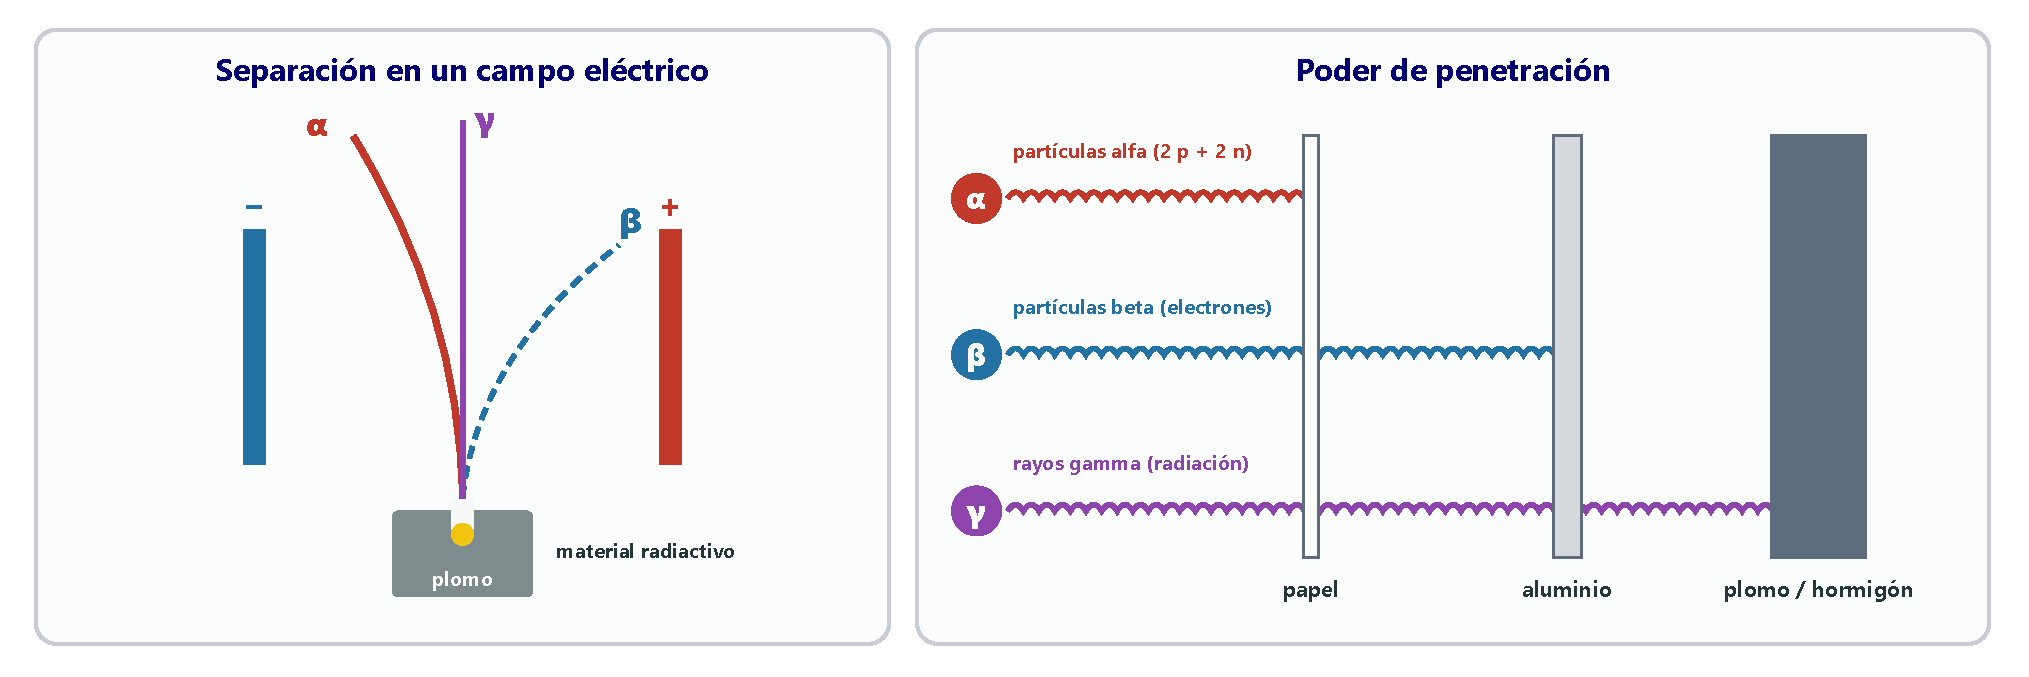
\includegraphics[width=\textwidth]{images/UD2/radiactividad}
    \caption{Comportamiento de las radiaciones \(\alpha\), \(\beta\) y \(\gamma\) en un campo eléctrico y su poder de penetración.}
    \label{fig:radiactividad}
\end{figure}

\begin{exercise}
    Investiga y describe tres aplicaciones de la radiactividad en medicina y otras dos en otros campos (industria, arqueología, energía…).
    \begin{solu}
        Respuesta libre. Por ejemplo: en medicina, la radioterapia contra el cáncer, los contrastes radiactivos para diagnóstico (gammagrafías, PET) y la esterilización de material quirúrgico. En otros campos: la datación por carbono-14 en arqueología, el control de soldaduras en la industria o la producción de energía en las centrales nucleares.
    \end{solu}
\end{exercise}

\begin{exercise}
    ¿Qué significaba originalmente la palabra «átomo»? ¿Quiénes la utilizaron por primera vez?
    \begin{solu}
        Significa «indivisible», «que no se puede dividir». La utilizaron por primera vez los filósofos griegos Leucipo y Demócrito, en el siglo \textsc{v}-\textsc{iv} a.\,C.
    \end{solu}
\end{exercise}

\begin{exercise}
    Escribe con tus propias palabras los postulados de la teoría atómica de Dalton. ¿Cuál de ellos tuvo que abandonarse primero?
    \begin{solu}
        Respuesta libre (ver los cuatro postulados del apartado 1.1). El primero que tuvo que abandonarse fue el de que los átomos son indivisibles, tras el descubrimiento del electrón y del protón.
    \end{solu}
\end{exercise}

\begin{exercise}
    ¿En qué experimentos se descubrieron el electrón y el protón? ¿Por qué fue tan importante este descubrimiento para la teoría atómica?
    \begin{solu}
        En los experimentos con tubos de descarga de gases (rayos catódicos y rayos canales). Fue importante porque demostró que el átomo es divisible: está formado por partículas más pequeñas con carga eléctrica.
    \end{solu}
\end{exercise}

\begin{exercise}
    ¿Cómo explicaba el modelo de Thomson que el átomo tuviera cargas positivas y negativas y que, aun así, fuera neutro?
    \begin{solu}
        Con el modelo del «pastel de pasas»: una esfera de carga positiva repartida uniformemente con los electrones incrustados en ella. La carga positiva de la esfera es igual a la suma de las cargas negativas de los electrones, por lo que el conjunto es neutro.
    \end{solu}
\end{exercise}

\begin{exercise}
    Indica cuáles de estas afirmaciones son falsas y corrígelas:
    \begin{enumerate}[label=\alph*)]
        \item En un átomo neutro hay tantos electrones como protones.
        \item El neutrón no tiene carga y su masa es menor que la del protón.
        \item Casi toda la masa del átomo se debe a los protones y los neutrones.
        \item El electrón es más pesado que el protón.
        \item El neutrón fue la última de las tres partículas en descubrirse.
        \item El protón y el electrón tienen cargas del mismo valor, pero de signo opuesto.
        \item Protones y neutrones se encuentran en el núcleo.
    \end{enumerate}
    \begin{solu}
        \begin{enumerate}[label=\alph*)]
            \item Verdadera.
            \item \textcolor{red}{Falsa.} El neutrón no tiene carga y su masa es \textbf{ligeramente mayor} que la del protón.
            \item Verdadera.
            \item \textcolor{red}{Falsa.} El protón es unas 1\,836 veces \textbf{más pesado} que el electrón.
            \item Verdadera (Chadwick, 1932).
            \item Verdadera.
            \item Verdadera.
        \end{enumerate}
    \end{solu}
\end{exercise}

\begin{exercise}
    Completa el texto sobre el modelo de Rutherford con las palabras: \emph{electrones, protones, neutrones, núcleo}.

    «Según Rutherford, el átomo es fundamentalmente un espacio vacío con un \rule{1.5cm}{0.4pt} central donde se concentra casi toda su masa, que se debe a los \rule{1.5cm}{0.4pt} y los \rule{1.5cm}{0.4pt}. La carga positiva también está en el \rule{1.5cm}{0.4pt}. Los \rule{1.5cm}{0.4pt} giran a gran velocidad a su alrededor y muy alejados de él.»
    \begin{solu}
        «\ldots con un \textcolor{red}{núcleo} central donde se concentra casi toda su masa, que se debe a los \textcolor{red}{protones} y los \textcolor{red}{neutrones}. La carga positiva también está en el \textcolor{red}{núcleo}. Los \textcolor{red}{electrones} giran a gran velocidad a su alrededor\ldots»
    \end{solu}
\end{exercise}

\begin{exercise}
    Sobre la radiactividad:
    \begin{enumerate}[label=\alph*)]
        \item ¿Qué tipos de partículas y radiaciones emiten las sustancias radiactivas?
        \item Describe brevemente las características de cada una.
        \item Si la radiactividad tiene lugar en el núcleo, ¿cómo es posible que se emitan electrones, si en el núcleo no hay electrones?
    \end{enumerate}
    \begin{solu}
        \begin{enumerate}[label=\alph*)]
            \item Partículas alfa, partículas beta y rayos gamma.
            \item Alfa: 2 protones y 2 neutrones, carga positiva, poco penetrantes (las detiene el papel). Beta: electrones rápidos, más penetrantes (las detiene una lámina de aluminio). Gamma: radiación de alta energía sin carga, muy penetrante (la detienen el plomo o el hormigón).
            \item Porque en el núcleo un neutrón se transforma en un protón y un electrón; el protón se queda en el núcleo y el electrón sale despedido como partícula beta.
        \end{enumerate}
    \end{solu}
\end{exercise}

\begin{exercise}
    Utiliza el modelo de Rutherford para explicar, con ayuda de un dibujo:
    \begin{enumerate}[label=\alph*)]
        \item Por qué una varilla de vidrio se carga al frotarla con un paño.
        \item Cómo se forman un ion positivo y un ion negativo.
    \end{enumerate}
    \begin{solu}
        \begin{enumerate}[label=\alph*)]
            \item Al frotar, algunos electrones pasan del vidrio al paño. El vidrio queda con menos electrones que protones (carga positiva) y el paño con más electrones que protones (carga negativa). Los protones no se mueven.
            \item Un átomo neutro que pierde electrones queda con más protones que electrones: catión (positivo). Si gana electrones, queda con más electrones que protones: anión (negativo). Ver la figura \ref{fig:iones}.
        \end{enumerate}
    \end{solu}
\end{exercise}

%========================================================================================
\section{¿Cómo identificamos los átomos de cada elemento?}
%========================================================================================

Cada átomo tiene una especie de «tarjeta de identidad». Lo que distingue a un átomo de calcio de uno de oxígeno o de hierro es el \textbf{número de protones} de su núcleo, que es siempre el mismo para todos los átomos de un elemento.

\subsection{El número atómico}

\begin{definition}[Número atómico, \(Z\)]
    Es el \textbf{número de protones} que hay en el núcleo de un átomo. Es un número entero y caracteriza al elemento: todos los átomos de un mismo elemento tienen el mismo \(Z\), y dos elementos distintos nunca tienen el mismo.
\end{definition}

Se escribe como subíndice a la izquierda del símbolo: \ch{_{11}Na}, \ch{_{8}O}. En un \textbf{átomo neutro}, el número de electrones es igual al de protones, así que \(Z\) también indica cuántos electrones tiene.

\subsection{El número másico}

\begin{definition}[Número másico, \(A\)]
    Es la \textbf{suma del número de protones y de neutrones} del núcleo. También es un número entero y se escribe como superíndice a la izquierda del símbolo: \ch{^{23}Na}, \ch{^{16}O}.
\end{definition}

\begin{figure}[H]
    \centering
    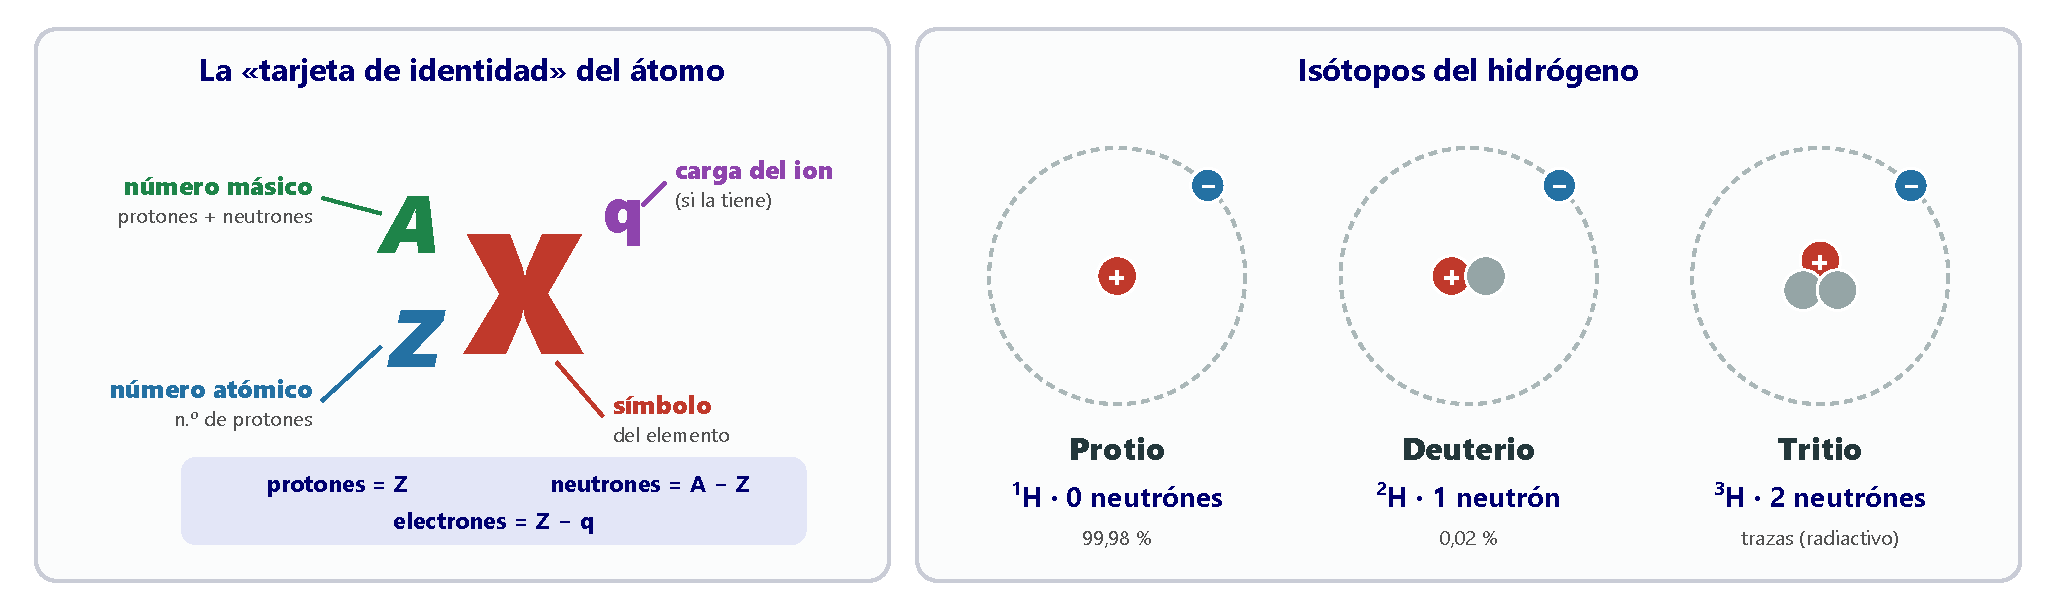
\includegraphics[width=\textwidth]{images/UD2/notacion_isotopos}
    \caption{Notación completa de un átomo o ion y los tres isótopos del hidrógeno.}
    \label{fig:notacion}
\end{figure}

A partir de \(Z\), \(A\) y la carga \(q\) del ion podemos contar todas las partículas:
\begin{centeredequation*}
    \text{protones} = Z \qquad \text{neutrones} = A - Z \qquad \text{electrones} = Z - q
\end{centeredequation*}

\begin{definition}[Isótopos]
    Son átomos de un mismo elemento que tienen el \textbf{mismo número atómico} (mismos protones), pero \textbf{distinto número másico}, porque tienen distinto número de neutrones.
\end{definition}

El número atómico de un elemento solo tiene un valor, pero el número másico puede tener varios, uno por cada isótopo. Por ejemplo, el hidrógeno tiene tres isótopos: protio (\ch{^1H}), deuterio (\ch{^2H}) y tritio (\ch{^3H}).

\begin{remark}
    \textbf{Radioisótopos.} Algunos isótopos tienen núcleos inestables y son radiactivos: se llaman \textbf{radioisótopos}. Por ejemplo, el carbono-14 (\ch{^{14}C}) es un isótopo radiactivo del carbono-12 (\ch{^{12}C}); se usa para datar restos arqueológicos.
\end{remark}

\begin{example}
    \textbf{Electrones de un catión y de un anión.}
    \begin{itemize}
        \item El sodio tiene \(Z = 11\). El átomo neutro tiene 11 protones y 11 electrones. Si pierde un electrón se convierte en el catión \ch{Na+}: sigue teniendo \textbf{11 protones}, pero ahora tiene \textbf{10 electrones}.
        \item El cloro tiene \(Z = 17\). Si un átomo neutro (17 protones, 17 electrones) gana un electrón, se forma el anión \ch{Cl-}: \textbf{17 protones} y \textbf{18 electrones}.
    \end{itemize}
\end{example}

\begin{exercise}
    ¿Es cierta esta frase? Justifica la respuesta: «Un catión y un anión tienen el mismo número de protones y de electrones que el átomo neutro del que proceden».
    \begin{solu}
        \textcolor{red}{Es falsa.} Los iones tienen el mismo número de \textbf{protones} que el átomo neutro, pero distinto número de \textbf{electrones}: el catión tiene menos y el anión tiene más.
    \end{solu}
\end{exercise}

\begin{exercise}
    El cloro tiene dos isótopos naturales, \ch{^{35}_{17}Cl} y \ch{^{37}_{17}Cl}. ¿Cuántos protones, neutrones y electrones tiene un átomo neutro de cloro-37?
    \begin{solu}
        \textcolor{blue}{Protones: \(Z = 17\). Electrones: 17 (es neutro). Neutrones: \(A - Z = 37 - 17\).}

        \textcolor{red}{17 protones, 20 neutrones y 17 electrones.}
    \end{solu}
\end{exercise}

\begin{exercise}
    Calcula el número de protones, neutrones y electrones de estas especies:
    \begin{multicols}{4}
        \begin{enumerate}[label=\alph*)]
            \item \ch{^{79}_{35}Br-}
            \item \ch{^{32}_{16}S^{2-}}
            \item \ch{^{27}_{13}Al^{3+}}
            \item \ch{^{207}_{82}Pb^{4+}}
        \end{enumerate}
    \end{multicols}
    \begin{solu}
        \begin{enumerate}[label=\alph*)]
            \item \ch{^{79}_{35}Br-}: 35 protones, \(79 - 35 = 44\) neutrones, \(35 + 1 = 36\) electrones.
            \item \ch{^{32}_{16}S^{2-}}: 16 protones, 16 neutrones, 18 electrones.
            \item \ch{^{27}_{13}Al^{3+}}: 13 protones, 14 neutrones, 10 electrones.
            \item \ch{^{207}_{82}Pb^{4+}}: 82 protones, 125 neutrones, 78 electrones.
        \end{enumerate}
    \end{solu}
\end{exercise}

\begin{exercise}
    Explica la diferencia entre número atómico y número másico. ¿Por qué los dos son siempre números enteros? ¿Podrían ser decimales?
    \begin{solu}
        El número atómico es el número de protones; el número másico es la suma de protones y neutrones. Son enteros porque cuentan partículas y no existen «trozos» de protón o de neutrón. Por tanto, nunca pueden ser decimales.
    \end{solu}
\end{exercise}

\begin{exercise}
    ¿Cómo se llama el número de protones de un átomo? ¿Pueden dos átomos de elementos distintos tener el mismo número de protones?
    \begin{solu}
        Se llama número atómico. No: si dos átomos tienen el mismo número de protones, son del mismo elemento.
    \end{solu}
\end{exercise}

\begin{exercise}
    ¿Qué es el número másico? ¿Pueden dos átomos de un mismo elemento tener distinto número másico? ¿Cómo se llaman?
    \begin{solu}
        Es la suma de protones y neutrones del núcleo. Sí: tienen los mismos protones pero distinto número de neutrones. Se llaman isótopos.
    \end{solu}
\end{exercise}

\begin{exercise}
    Copia y completa la tabla en tu cuaderno:
    \begin{center}
        % --- tabla antigua ---
        % \begin{tblr}{colspec={cccc}, hlines, vlines, row{1}={bg=ocre!85, fg=white, font=\bfseries}}
            % Átomo & Protones & Electrones & Neutrones \\
            % \ch{^{107}_{47}Ag} & & & \\
            % \ch{^{206}_{82}Pb} & & & \\
            % \ch{^{133}_{55}Cs} & & & \\
            % \ch{^{71}_{31}Ga} & & & \\
        % \end{tblr}
        % --- tabla nueva ---
        \begin{tabular}{@{}cccc@{}}
            \toprule
            \textbf{Átomo} & \textbf{Protones} & \textbf{Electrones} & \textbf{Neutrones} \\
            \midrule
            \ch{^{107}_{47}Ag} &  &  &  \\[3pt]
            \ch{^{206}_{82}Pb} &  &  &  \\[3pt]
            \ch{^{133}_{55}Cs} &  &  &  \\[3pt]
            \ch{^{71}_{31}Ga} &  &  &  \\
            \bottomrule
        \end{tabular}
    \end{center}
    \begin{solu}
        \begin{center}
            % --- tabla antigua ---
            % \begin{tblr}{colspec={cccc}, hlines, vlines, row{1}={font=\bfseries}}
                % Átomo & Protones & Electrones & Neutrones \\
                % \ch{^{107}_{47}Ag} & 47 & 47 & 60 \\
                % \ch{^{206}_{82}Pb} & 82 & 82 & 124 \\
                % \ch{^{133}_{55}Cs} & 55 & 55 & 78 \\
                % \ch{^{71}_{31}Ga} & 31 & 31 & 40 \\
            % \end{tblr}
            % --- tabla nueva ---
            \begin{tabular}{@{}cccc@{}}
                \toprule
                \textbf{Átomo} & \textbf{Protones} & \textbf{Electrones} & \textbf{Neutrones} \\
                \midrule
                \ch{^{107}_{47}Ag} & 47 & 47 & 60 \\[3pt]
                \ch{^{206}_{82}Pb} & 82 & 82 & 124 \\[3pt]
                \ch{^{133}_{55}Cs} & 55 & 55 & 78 \\[3pt]
                \ch{^{71}_{31}Ga} & 31 & 31 & 40 \\
                \bottomrule
            \end{tabular}
        \end{center}
    \end{solu}
\end{exercise}

\begin{exercise}
    Completa la tabla para estos iones:
    \begin{center}
        % --- tabla antigua ---
        % \begin{tblr}{colspec={cccc}, hlines, vlines, row{1}={bg=ocre!85, fg=white, font=\bfseries}}
            % Ion & Protones & Electrones & Neutrones \\
            % \ch{^{4}_{2}He^{2+}} & & & \\
            % \ch{^{16}_{8}O^{2-}} & & & \\
            % \ch{^{23}_{11}Na+} & & & \\
            % \ch{^{81}_{35}Br-} & & & \\
            % \ch{^{24}_{12}Mg^{2+}} & & & \\
            % \ch{^{106}_{46}Pd^{4+}} & & & \\
            % \ch{^{75}_{33}As^{3-}} & & & \\
        % \end{tblr}
        % --- tabla nueva ---
        \begin{tabular}{@{}cccc@{}}
            \toprule
            \textbf{Ion} & \textbf{Protones} & \textbf{Electrones} & \textbf{Neutrones} \\
            \midrule
            \ch{^{4}_{2}He^{2+}} &  &  &  \\[3pt]
            \ch{^{16}_{8}O^{2-}} &  &  &  \\[3pt]
            \ch{^{23}_{11}Na+} &  &  &  \\[3pt]
            \ch{^{81}_{35}Br-} &  &  &  \\[3pt]
            \ch{^{24}_{12}Mg^{2+}} &  &  &  \\[3pt]
            \ch{^{106}_{46}Pd^{4+}} &  &  &  \\[3pt]
            \ch{^{75}_{33}As^{3-}} &  &  &  \\
            \bottomrule
        \end{tabular}
    \end{center}
    \begin{solu}
        \begin{center}
            % --- tabla antigua ---
            % \begin{tblr}{colspec={cccc}, hlines, vlines, row{1}={font=\bfseries}}
                % Ion & Protones & Electrones & Neutrones \\
                % \ch{^{4}_{2}He^{2+}} & 2 & 0 & 2 \\
                % \ch{^{16}_{8}O^{2-}} & 8 & 10 & 8 \\
                % \ch{^{23}_{11}Na+} & 11 & 10 & 12 \\
                % \ch{^{81}_{35}Br-} & 35 & 36 & 46 \\
                % \ch{^{24}_{12}Mg^{2+}} & 12 & 10 & 12 \\
                % \ch{^{106}_{46}Pd^{4+}} & 46 & 42 & 60 \\
                % \ch{^{75}_{33}As^{3-}} & 33 & 36 & 42 \\
            % \end{tblr}
            % --- tabla nueva ---
            \begin{tabular}{@{}cccc@{}}
                \toprule
                \textbf{Ion} & \textbf{Protones} & \textbf{Electrones} & \textbf{Neutrones} \\
                \midrule
                \ch{^{4}_{2}He^{2+}} & 2 & 0 & 2 \\[3pt]
                \ch{^{16}_{8}O^{2-}} & 8 & 10 & 8 \\[3pt]
                \ch{^{23}_{11}Na+} & 11 & 10 & 12 \\[3pt]
                \ch{^{81}_{35}Br-} & 35 & 36 & 46 \\[3pt]
                \ch{^{24}_{12}Mg^{2+}} & 12 & 10 & 12 \\[3pt]
                \ch{^{106}_{46}Pd^{4+}} & 46 & 42 & 60 \\[3pt]
                \ch{^{75}_{33}As^{3-}} & 33 & 36 & 42 \\
                \bottomrule
            \end{tabular}
        \end{center}
    \end{solu}
\end{exercise}

\begin{exercise}
    Observa estos átomos imaginarios (las letras no son símbolos reales):
    \[ \ch{^{50}_{25}A} \quad \ch{^{39}_{19}C} \quad \ch{^{52}_{25}E} \quad \ch{^{102}_{49}G} \quad \ch{^{10}_{5}I} \quad \ch{^{29}_{14}B} \quad \ch{^{110}_{51}D} \quad \ch{^{40}_{19}F} \quad \ch{^{28}_{14}H} \quad \ch{^{51}_{25}J} \]
    \begin{enumerate}[label=\alph*)]
        \item Agrupa los que sean isótopos entre sí.
        \item Indica el número de protones y de neutrones de cada uno de esos isótopos.
        \item ¿En qué se diferencian los isótopos de un mismo grupo?
    \end{enumerate}
    \begin{solu}
        \begin{enumerate}[label=\alph*)]
            \item Son isótopos los que tienen el mismo \(Z\): A, E y J (\(Z = 25\)); B y H (\(Z = 14\)); C y F (\(Z = 19\)).
            \item A, E y J: 25 protones y 25, 27 y 26 neutrones, respectivamente. B y H: 14 protones y 15 y 14 neutrones. C y F: 19 protones y 20 y 21 neutrones.
            \item En el número de neutrones y, por tanto, en el número másico.
        \end{enumerate}
    \end{solu}
\end{exercise}

%========================================================================================
\section{¿Cómo se mide la masa de un átomo? La masa atómica}
%========================================================================================

Un átomo de carbono tiene una masa de unos \qty{2e-26}{\kg}. El kilogramo es una unidad enorme para medir algo tan pequeño, así que los químicos utilizan una unidad mucho más adecuada.

\begin{definition}[Unidad de masa atómica, u]
    Es la \textbf{doceava parte} de la masa de un átomo de carbono-12 (\ch{^{12}C}). Equivale aproximadamente a \qty{1.66e-27}{\kg}.
\end{definition}

\begin{figure}[H]
    \centering
    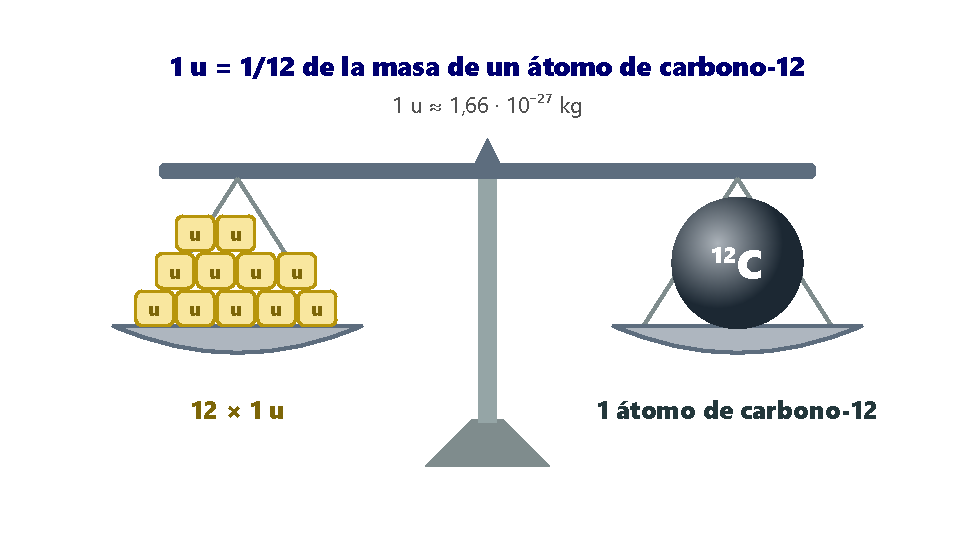
\includegraphics[width=0.6\textwidth]{images/UD2/masa_atomica_balanza}
    \caption{Hacen falta 12 unidades de masa atómica para «equilibrar» un átomo de carbono-12: su masa atómica es 12.}
    \label{fig:balanza}
\end{figure}

\begin{definition}[Masa atómica relativa, \(A_r\)]
    Es la masa de un átomo comparada con la doceava parte de la masa del átomo de carbono-12. Es una magnitud \textbf{adimensional} (no tiene unidades). Se le suele llamar simplemente \textbf{masa atómica}.
\end{definition}

Decir que la masa atómica relativa del oxígeno es 16 significa que un átomo de oxígeno tiene 16 veces más masa que la doceava parte de un átomo de carbono-12.

\subsection{¿Cómo se calcula la masa atómica de un elemento?}

\begin{itemize}
    \item Si el elemento solo tiene \textbf{un isótopo natural} (es \textbf{monoisotópico}), su masa atómica coincide con la de ese isótopo. Por ejemplo, todo el sodio natural es Na-23, así que su masa atómica es 23.
    \item Si el elemento tiene \textbf{varios isótopos}, su masa atómica es la \textbf{media ponderada} de las masas de sus isótopos según su abundancia. Por eso casi nunca es un número entero:
\end{itemize}

\begin{centeredequation}
    A_r = m_1 \cdot \frac{\%_1}{100} + m_2 \cdot \frac{\%_2}{100} + \dots
\end{centeredequation}

donde \(m_1\), \(m_2\)\ldots{} son las masas atómicas relativas de cada isótopo y \(\%_1\), \(\%_2\)\ldots{} sus abundancias. Si no se indica otra cosa, se puede tomar como masa de cada isótopo su número másico.

\begin{example}
    \textbf{Masa atómica del oxígeno.} El oxígeno natural está formado por tres isótopos: oxígeno-16 (\qty{99.759}{\percent}), oxígeno-17 (\qty{0.037}{\percent}) y oxígeno-18 (\qty{0.204}{\percent}). Calcula su masa atómica relativa.

    \textcolor{blue}{Multiplicamos la masa de cada isótopo por su abundancia y sumamos:}
    \[ A_r(\ch{O}) = \frac{16 \cdot \num{99.759} + 17 \cdot \num{0.037} + 18 \cdot \num{0.204}}{100} = \textcolor{red}{\num{16.004}} \]
\end{example}

\begin{exercise}
    Un elemento imaginario está formado por dos isótopos, X-63 y X-65. Si el \qty{60}{\percent} de sus átomos son del primero, ¿cuál es su masa atómica relativa?
    \begin{solu}
        \[ A_r = 63 \cdot \frac{60}{100} + 65 \cdot \frac{40}{100} = \num{37.8} + 26 = \textcolor{red}{\num{63.8}} \]
    \end{solu}
\end{exercise}

\begin{exercise}
    El cobre tiene una masa atómica relativa de \num{63.546} y está formado por dos isótopos de masas \num{62.9298} y \num{64.9278}. Calcula el porcentaje de cada isótopo en el cobre natural.
    \begin{solu}
        \textcolor{blue}{Llamamos \(x\) a la fracción del primer isótopo; la del segundo es \(1 - x\):}
        \[ \num{62.9298}\,x + \num{64.9278}\,(1 - x) = \num{63.546} \;\Rightarrow\; x = \frac{\num{64.9278} - \num{63.546}}{\num{64.9278} - \num{62.9298}} = \num{0.6916} \]
        \textcolor{red}{Cu-63: \qty{69.16}{\percent}; Cu-65: \qty{30.84}{\percent}.}
    \end{solu}
\end{exercise}

\begin{exercise}
    Un elemento tiene una masa atómica relativa de \num{85.47} y está formado por dos isótopos de masas 85 y 87. Calcula el porcentaje de cada uno.
    \begin{solu}
        \[ 85\,x + 87\,(1 - x) = \num{85.47} \;\Rightarrow\; 87 - 2x = \num{85.47} \;\Rightarrow\; x = \num{0.765} \]
        \textcolor{red}{Isótopo de masa 85: \qty{76.5}{\percent}; isótopo de masa 87: \qty{23.5}{\percent}.}
    \end{solu}
\end{exercise}

\begin{exercise}
    La masa atómica relativa del níquel es \num{58.71}. Suponiendo que solo tuviera dos isótopos, de masas 58 y 60, ¿en qué porcentaje se encontraría cada uno?
    \begin{solu}
        \[ 58\,x + 60\,(1 - x) = \num{58.71} \;\Rightarrow\; 60 - 2x = \num{58.71} \;\Rightarrow\; x = \num{0.645} \]
        \textcolor{red}{Ni-58: \qty{64.5}{\percent}; Ni-60: \qty{35.5}{\percent}.}
    \end{solu}
\end{exercise}

\begin{exercise}
    La masa atómica relativa del cloro es \num{35.45}. Sabiendo que está formado por cloro-35 y cloro-37, calcula la abundancia de cada isótopo.
    \begin{solu}
        \[ 35\,x + 37\,(1 - x) = \num{35.45} \;\Rightarrow\; 37 - 2x = \num{35.45} \;\Rightarrow\; x = \num{0.775} \]
        \textcolor{red}{Cl-35: \qty{77.5}{\percent}; Cl-37: \qty{22.5}{\percent}.}
    \end{solu}
\end{exercise}

\begin{exercise}
    El estroncio natural es una mezcla de cuatro isótopos. Con los datos de la tabla, calcula su masa atómica relativa.
    \begin{center}
        % --- tabla antigua ---
        % \begin{tblr}{colspec={ccc}, hlines, vlines, row{1}={bg=ocre!85, fg=white, font=\bfseries}}
            % Isótopo & Masa atómica relativa & Abundancia (\%) \\
            % Sr-84 & \num{83.9134} & \num{0.5} \\
            % Sr-86 & \num{85.9094} & \num{9.9} \\
            % Sr-87 & \num{86.9089} & \num{7.0} \\
            % Sr-88 & \num{87.9056} & \num{82.6} \\
        % \end{tblr}
        % --- tabla nueva ---
        \begin{tabular}{@{}ccc@{}}
            \toprule
            \textbf{Isótopo} & \textbf{Masa atómica relativa} & \textbf{Abundancia (\%)} \\
            \midrule
            Sr-84 & \num{83.9134} & \num{0.5} \\[3pt]
            Sr-86 & \num{85.9094} & \num{9.9} \\[3pt]
            Sr-87 & \num{86.9089} & \num{7.0} \\[3pt]
            Sr-88 & \num{87.9056} & \num{82.6} \\
            \bottomrule
        \end{tabular}
    \end{center}
    \begin{solu}
        \[ A_r = \num{83.9134}\cdot\num{0.005} + \num{85.9094}\cdot\num{0.099} + \num{86.9089}\cdot\num{0.070} + \num{87.9056}\cdot\num{0.826} = \textcolor{red}{\num{87.62}} \]
    \end{solu}
\end{exercise}

\begin{exercise}
    El magnesio tiene tres isótopos naturales. Calcula su masa atómica relativa con estos datos:
    \begin{center}
        % --- tabla antigua ---
        % \begin{tblr}{colspec={ccc}, hlines, vlines, row{1}={bg=ocre!85, fg=white, font=\bfseries}}
            % Isótopo & Masa atómica relativa & Abundancia (\%) \\
            % Mg-24 & \num{23.8850} & \num{78.99} \\
            % Mg-25 & \num{24.9858} & \num{10.00} \\
            % Mg-26 & \num{25.9826} & \num{11.01} \\
        % \end{tblr}
        % --- tabla nueva ---
        \begin{tabular}{@{}ccc@{}}
            \toprule
            \textbf{Isótopo} & \textbf{Masa atómica relativa} & \textbf{Abundancia (\%)} \\
            \midrule
            Mg-24 & \num{23.8850} & \num{78.99} \\[3pt]
            Mg-25 & \num{24.9858} & \num{10.00} \\[3pt]
            Mg-26 & \num{25.9826} & \num{11.01} \\
            \bottomrule
        \end{tabular}
    \end{center}
    \begin{solu}
        \[ A_r = \num{23.8850}\cdot\num{0.7899} + \num{24.9858}\cdot\num{0.1000} + \num{25.9826}\cdot\num{0.1101} = \textcolor{red}{\num{24.23}} \]
    \end{solu}
\end{exercise}

\begin{exercise}
    El uranio natural contiene un \qty{0.0057}{\percent} de uranio-234, un \qty{0.72}{\percent} de uranio-235 y un \qty{99.27}{\percent} de uranio-238. ¿Cuál es su masa atómica relativa?
    \begin{solu}
        \[ A_r = 234\cdot\num{0.000057} + 235\cdot\num{0.0072} + 238\cdot\num{0.9927} = \textcolor{red}{\num{237.97}} \]
    \end{solu}
\end{exercise}

%========================================================================================
\section{Los espectros atómicos}
%========================================================================================

Estudiar la luz que emiten o absorben los átomos ha sido una de las herramientas más útiles para conocer cómo son por dentro.

Cuando un haz de \textbf{luz blanca} atraviesa un prisma de vidrio, se separa en todos los colores que la forman, del rojo al violeta, sin saltos entre ellos: es un \textbf{espectro continuo}.

\subsection{¿Cómo se forma un espectro discontinuo?}

Un \textbf{espectroscopio} es un aparato que analiza la luz emitida por los átomos de un elemento previamente excitados (calentándolos o mediante una descarga eléctrica). Al estudiar así los elementos químicos se descubrió algo sorprendente: su luz \textbf{no} forma un espectro continuo, sino un conjunto de \textbf{rayas} separadas. Los espectros atómicos son \textbf{discontinuos}.

\begin{itemize}
    \item \negsubro{Espectro de emisión.} Es el conjunto de radiaciones que emiten los átomos de un elemento excitado. Se ve como rayas de colores sobre fondo negro.
    \item \negsubro{Espectro de absorción.} Se obtiene al hacer pasar luz blanca a través del elemento (en estado gaseoso). Aparece el arco iris con \textbf{rayas oscuras}: son las radiaciones que el elemento ha absorbido, y están en las \textbf{mismas posiciones} que las rayas luminosas de su espectro de emisión.
\end{itemize}

\begin{figure}[H]
    \centering
    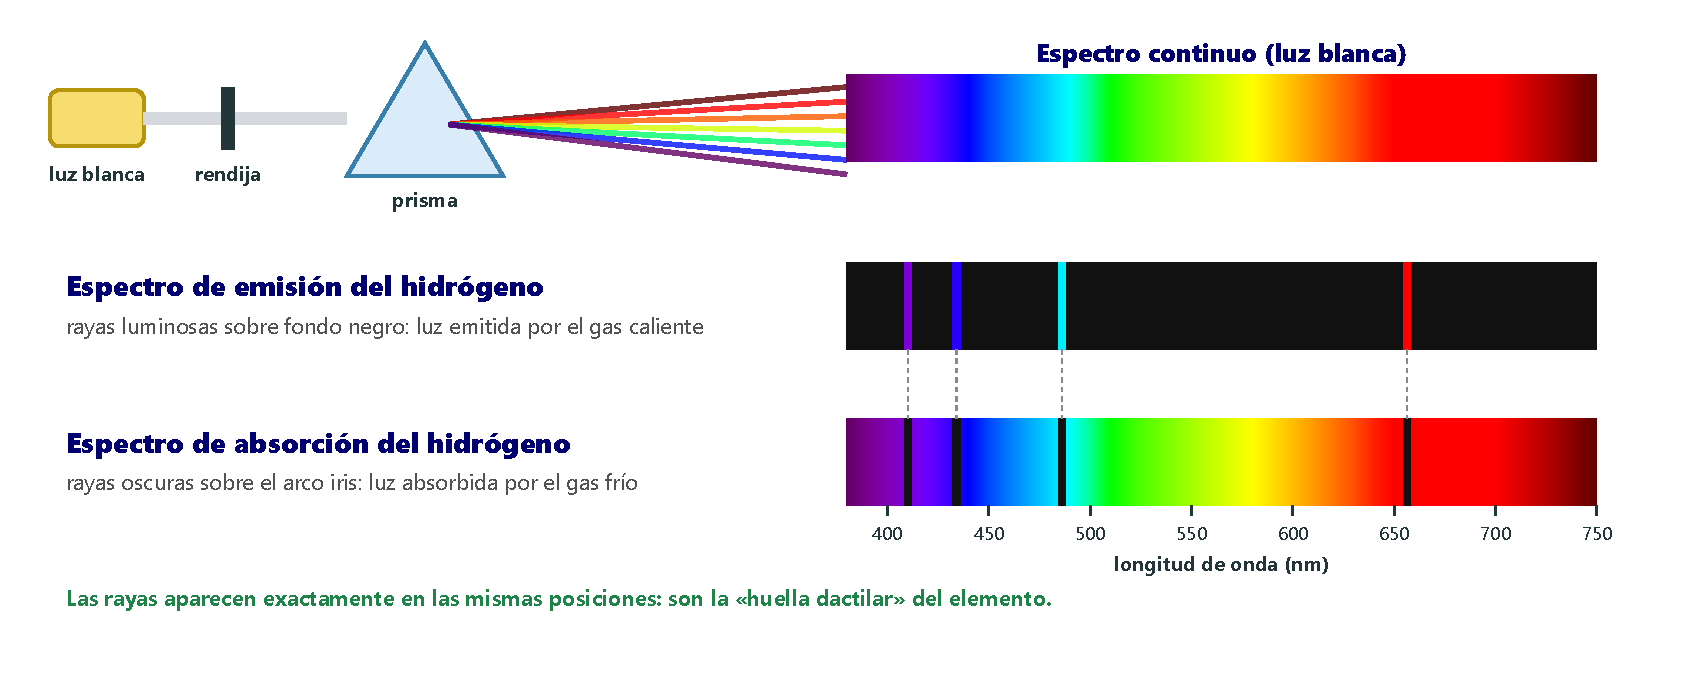
\includegraphics[width=\textwidth]{images/UD2/espectros}
    \caption{Espectro continuo de la luz blanca y espectros de emisión y absorción del hidrógeno.}
    \label{fig:espectros}
\end{figure}

\begin{remark}
    El espectro de cada elemento es \textbf{único}, distinto del de cualquier otro: es su \textbf{«huella dactilar»}. Gracias a ello podemos saber de qué está hecha una estrella sin viajar hasta ella. El helio se descubrió en 1868 en el espectro del Sol, ¡antes que en la Tierra!
\end{remark}

\subsection{¿Por qué el modelo de Rutherford no pudo explicarlos?}

Según el electromagnetismo, una carga eléctrica que se mueve en círculo (y, por tanto, está acelerada) emite energía continuamente en forma de radiación. Si el modelo de Rutherford fuera correcto:
\begin{enumerate}[label=\numberballred]
    \item Los átomos emitirían todo tipo de radiaciones y sus espectros serían \textbf{continuos}, no de rayas.
    \item El electrón, al perder energía, se acercaría cada vez más al núcleo hasta \textbf{caer sobre él}, y el átomo no sería estable. Esto, evidentemente, no ocurre.
\end{enumerate}

\begin{figure}[H]
    \centering
    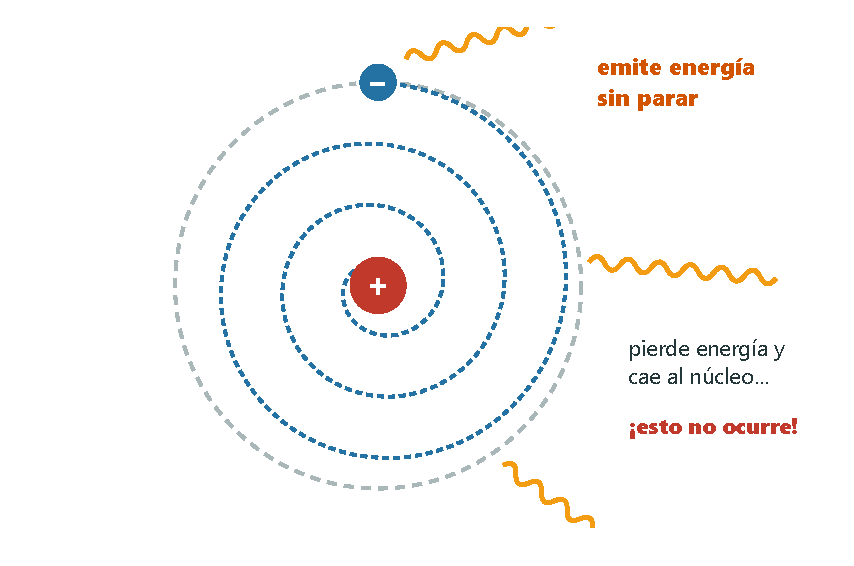
\includegraphics[width=0.5\textwidth]{images/UD2/fallo_rutherford}
    \caption{Según la física clásica, el electrón del modelo de Rutherford debería radiar energía y caer en espiral sobre el núcleo.}
    \label{fig:fallo_rutherford}
\end{figure}

\begin{exercise}
    Clasifica estos espectros en continuos o discontinuos y, en su caso, en espectros de emisión o de absorción:

    \begin{tabular}{rl}
        a) & \espectroabsorcion{0.12,0.2,0.36,0.52,0.6,0.86} \\[4pt]
        b) & \espectrocontinuo \\[4pt]
        c) & \espectroemision{0.18/blue,0.42/green!70!black,0.71/orange,0.83/red}
    \end{tabular}
    \begin{solu}
        \begin{enumerate}[label=\alph*)]
            \item Espectro discontinuo de absorción (rayas oscuras sobre el arco iris).
            \item Espectro continuo.
            \item Espectro discontinuo de emisión (rayas de colores sobre fondo negro).
        \end{enumerate}
    \end{solu}
\end{exercise}

\begin{exercise}
    ¿El espectro de la luz blanca es continuo o de rayas? ¿Y el de la luz emitida por un tubo con gas neón?
    \begin{solu}
        El de la luz blanca es continuo. El del neón, como el de cualquier elemento excitado, es un espectro de emisión de rayas (discontinuo).
    \end{solu}
\end{exercise}

\begin{exercise}
    ¿Es posible que dos elementos químicos distintos tengan exactamente el mismo espectro? Razona tu respuesta.
    \begin{solu}
        No. La distribución de rayas del espectro de cada elemento es única y diferente de la de todos los demás; por eso se usa para identificar elementos.
    \end{solu}
\end{exercise}

\begin{exercise}
    ¿Qué es un espectro atómico de emisión? Explica cómo podríamos obtener el de un elemento concreto.
    \begin{solu}
        Es el conjunto de radiaciones que emiten los átomos de un elemento que ha sido excitado previamente. Se obtiene calentando el elemento o sometiéndolo a una descarga eléctrica (por ejemplo, un gas en un tubo de descarga) y analizando la luz emitida con un espectroscopio.
    \end{solu}
\end{exercise}

\begin{exercise}
    Razona si estos dos espectros pueden pertenecer al mismo elemento:

    \begin{tabular}{rl}
        A & \espectroabsorcion{0.08,0.3,0.5,0.62,0.78,0.9} \\[4pt]
        B & \espectroemision{0.14/violet,0.36/cyan,0.68/orange,0.92/red}
    \end{tabular}
    \begin{solu}
        El A es de absorción y el B de emisión. Si fueran del mismo elemento, las rayas oscuras de A estarían exactamente en las mismas posiciones que las rayas luminosas de B. Como no coinciden, \textcolor{red}{son de elementos distintos}.
    \end{solu}
\end{exercise}

\begin{exercise}
    ¿Pertenecen estos dos espectros al mismo elemento? Indica cuál es de emisión y cuál de absorción.

    \begin{tabular}{rl}
        A & \espectroabsorcion{0.1,0.22,0.47,0.81} \\[4pt]
        B & \espectroemision{0.1/violet,0.22/blue,0.47/cyan,0.81/red}
    \end{tabular}
    \begin{solu}
        \textcolor{red}{Sí}: las rayas oscuras de A están en las mismas posiciones que las rayas luminosas de B. A es el espectro de absorción y B el de emisión.
    \end{solu}
\end{exercise}

%========================================================================================
\section{El modelo de los niveles de energía}
%========================================================================================

En 1913, el físico danés \textbf{Niels Bohr} propuso un nuevo modelo atómico, basado en la existencia de \textbf{niveles de energía} dentro del átomo. Con él explicó la estabilidad del átomo de hidrógeno y su espectro de rayas.

\subsection{Los postulados de Bohr}

\begin{itemize}
    \item \negsubro{Primer postulado.} El electrón solo puede girar en ciertas \textbf{órbitas circulares estables}, en las que se mueve a gran velocidad \textbf{sin emitir energía}. Así se resuelve el problema del modelo de Rutherford: el electrón no cae al núcleo.
    \item \negsubro{Segundo postulado.} En cada órbita, el electrón tiene una \textbf{energía determinada}, que es mayor cuanto más lejos del núcleo está la órbita. Cada órbita es un \textbf{nivel de energía} y se identifica por un número \(n = 1, 2, 3\ldots\)
    \item \negsubro{Tercer postulado.} Mientras está en una órbita estable el electrón no radia energía. Cuando \textbf{baja} de un nivel de mayor energía a otro de menor energía, \textbf{emite} la diferencia en forma de radiación; para \textbf{subir} a un nivel superior, necesita \textbf{absorber} energía.
\end{itemize}

Solo algunas órbitas están permitidas, y los niveles de energía son distintos en cada elemento; por eso sus espectros también lo son.

\subsection{¿Cómo explica el modelo de Bohr los espectros?}

Cuando un átomo recibe energía (por calor o una descarga eléctrica), algunos electrones \textbf{saltan} a niveles más alejados del núcleo. Al volver a niveles inferiores, emiten una energía \textbf{exactamente igual} a la diferencia entre los dos niveles. Por ejemplo, si el electrón pasa del nivel 5 al nivel 1:
\begin{centeredequation*}
    E_{\text{emitida}} = E_5 - E_1
\end{centeredequation*}

Como solo hay unos pocos saltos posibles, solo se emiten unas pocas energías concretas: cada salto produce \textbf{una raya} del espectro.

\begin{figure}[H]
    \centering
    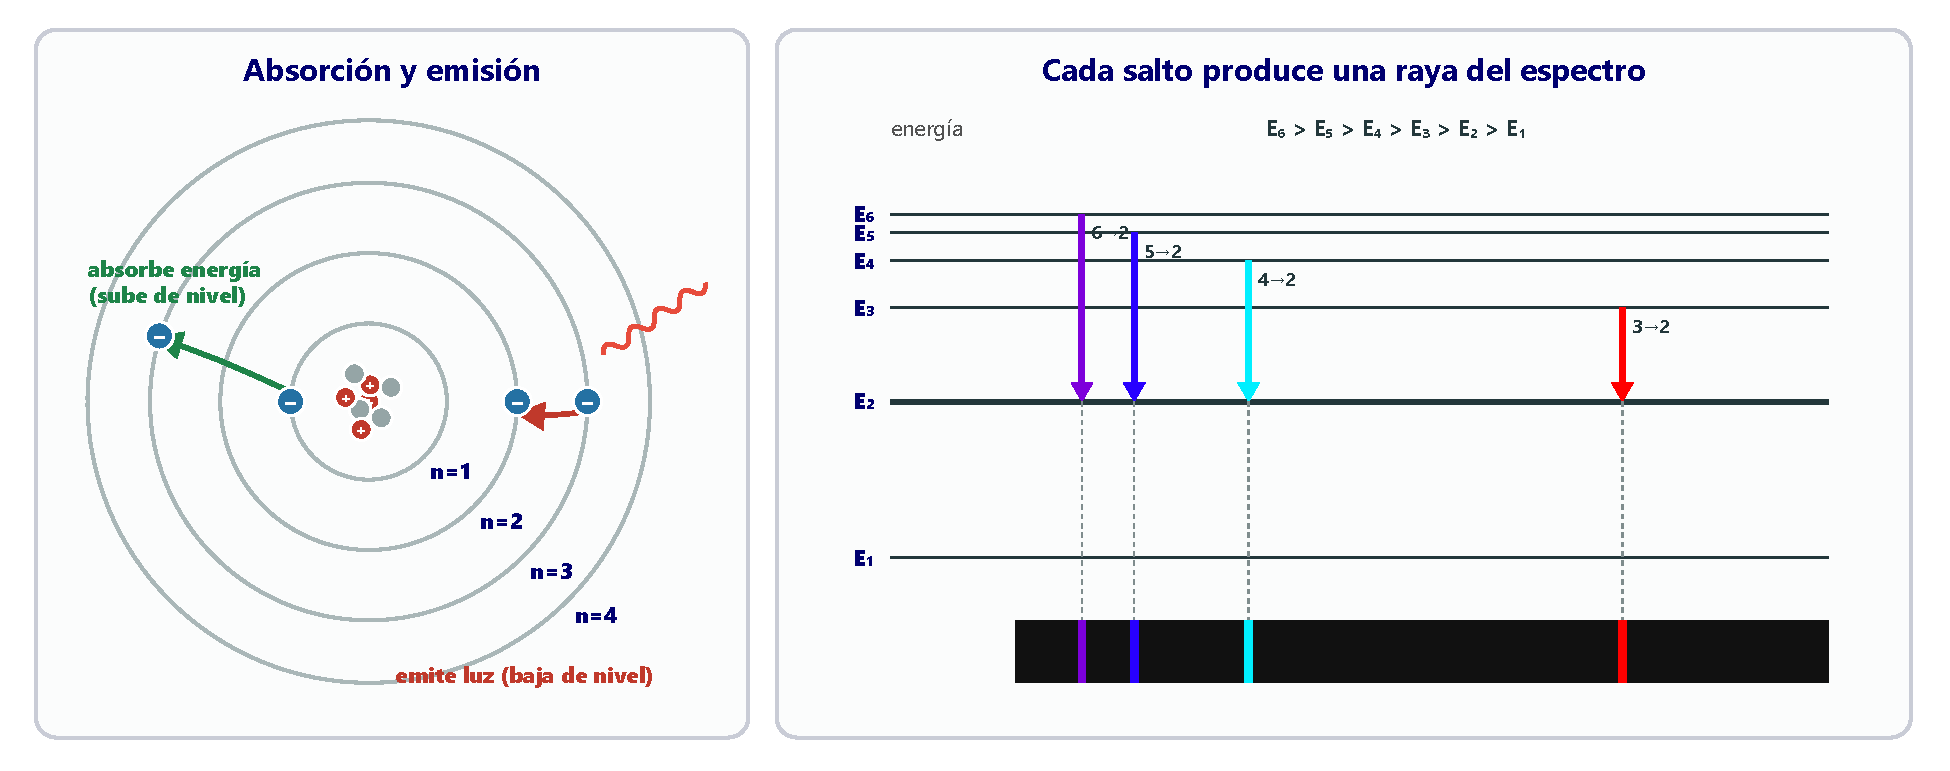
\includegraphics[width=\textwidth]{images/UD2/bohr_saltos}
    \caption{Según Bohr, cada raya del espectro de emisión corresponde a un salto del electrón desde un nivel de energía superior a otro inferior. Las cuatro rayas visibles del hidrógeno se deben a saltos que terminan en el nivel 2.}
    \label{fig:bohr_saltos}
\end{figure}

\subsection{Niveles y subniveles: el modelo de Bohr-Sommerfeld}

Cada nivel puede albergar un número máximo de electrones, que vale \(2n^2\): 2 en el nivel 1, 8 en el nivel 2, 18 en el nivel 3, 32 en el nivel 4\ldots

Con espectroscopios más precisos se vio que muchas rayas eran, en realidad, varias rayas muy juntas. Para explicarlo, \textbf{Arnold Sommerfeld} propuso en 1916 que cada nivel de energía está formado por varios \textbf{subniveles} muy próximos entre sí. Así hay más saltos posibles y aparecen más rayas en el espectro.

Los subniveles se nombran con las letras \textbf{s}, \textbf{p}, \textbf{d} y \textbf{f}, y cada uno admite un número máximo de electrones:

\begin{table}[H]
    \centering
    % --- tabla antigua ---
    % \begin{tblr}{colspec={cccc}, hlines, vlines, row{1}={bg=ocre!85, fg=white, font=\bfseries}, column{1}={bg=ocre!15, font=\bfseries}, cell{1}{1}={bg=ocre!85, fg=white},
        % cell{2}{4}={r=1}{c}, cell{3}{1}={r=2}{c}, cell{3}{4}={r=2}{c}, cell{5}{1}={r=3}{c}, cell{5}{4}={r=3}{c}, cell{8}{1}={r=4}{c}, cell{8}{4}={r=4}{c}}
        % Nivel (\(n\)) & Subniveles & Electrones por subnivel & Electrones por nivel (\(2n^2\)) \\
        % 1 & s & 2 & 2 \\
        % 2 & s & 2 & 8 \\
          % & p & 6 & \\
        % 3 & s & 2 & 18 \\
          % & p & 6 & \\
          % & d & 10 & \\
        % 4 & s & 2 & 32 \\
          % & p & 6 & \\
          % & d & 10 & \\
          % & f & 14 & \\
    % \end{tblr}
    % --- tabla nueva ---
    \begin{tabular}{@{}cccc@{}}
        \toprule
        \textbf{Nivel (\(n\))} & \textbf{Subniveles} & \textbf{Electrones por subnivel} & \textbf{Electrones por nivel (\(2n^2\))} \\
        \midrule
        \textbf{1} & s & 2 & 2 \\[3pt]
        \multirow{2}{*}{\textbf{2}} & s & 2 & \multirow{2}{*}{8} \\[3pt]
         & p & 6 &  \\[3pt]
        \multirow{3}{*}{\textbf{3}} & s & 2 & \multirow{3}{*}{18} \\[3pt]
         & p & 6 &  \\[3pt]
         & d & 10 &  \\[3pt]
        \multirow{4}{*}{\textbf{4}} & s & 2 & \multirow{4}{*}{32} \\[3pt]
         & p & 6 &  \\[3pt]
         & d & 10 &  \\[3pt]
         & f & 14 &  \\
        \bottomrule
    \end{tabular}
    \caption{Capacidad de los niveles y subniveles de energía.}
    \label{tab:subniveles}
\end{table}

\begin{figure}[H]
    \centering
    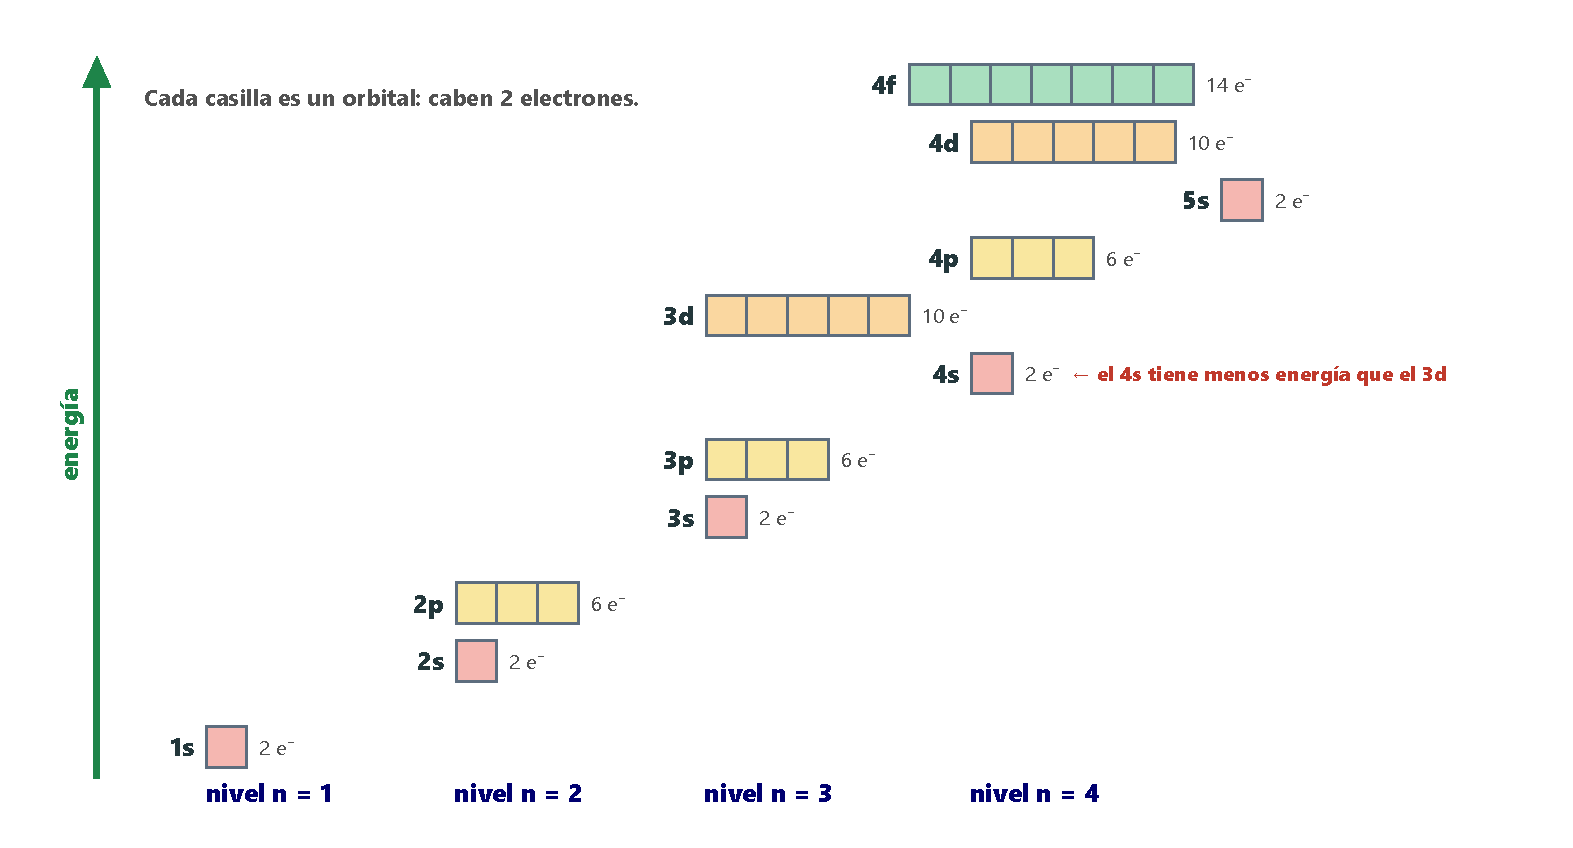
\includegraphics[width=\textwidth]{images/UD2/niveles_subniveles}
    \caption{Desdoblamiento de los niveles en subniveles. Cada casilla representa un orbital, con capacidad para dos electrones. Fíjate en que el subnivel 4s tiene menos energía que el 3d.}
    \label{fig:niveles_subniveles}
\end{figure}

\subsection{La configuración electrónica}

\begin{definition}[Configuración electrónica]
    Es la forma en que se distribuyen los electrones de un átomo en los distintos niveles y subniveles. Los electrones ocupan los subniveles \textbf{de menor a mayor energía}, sin superar la capacidad máxima de cada uno.
\end{definition}

El orden de energía de los subniveles no es simplemente 1, 2, 3\ldots: por ejemplo, el 4s se llena antes que el 3d. Para recordarlo se usa el \textbf{diagrama de Moeller}: se escriben los subniveles en filas y se recorren siguiendo las flechas diagonales.

\begin{figure}[H]
    \centering
    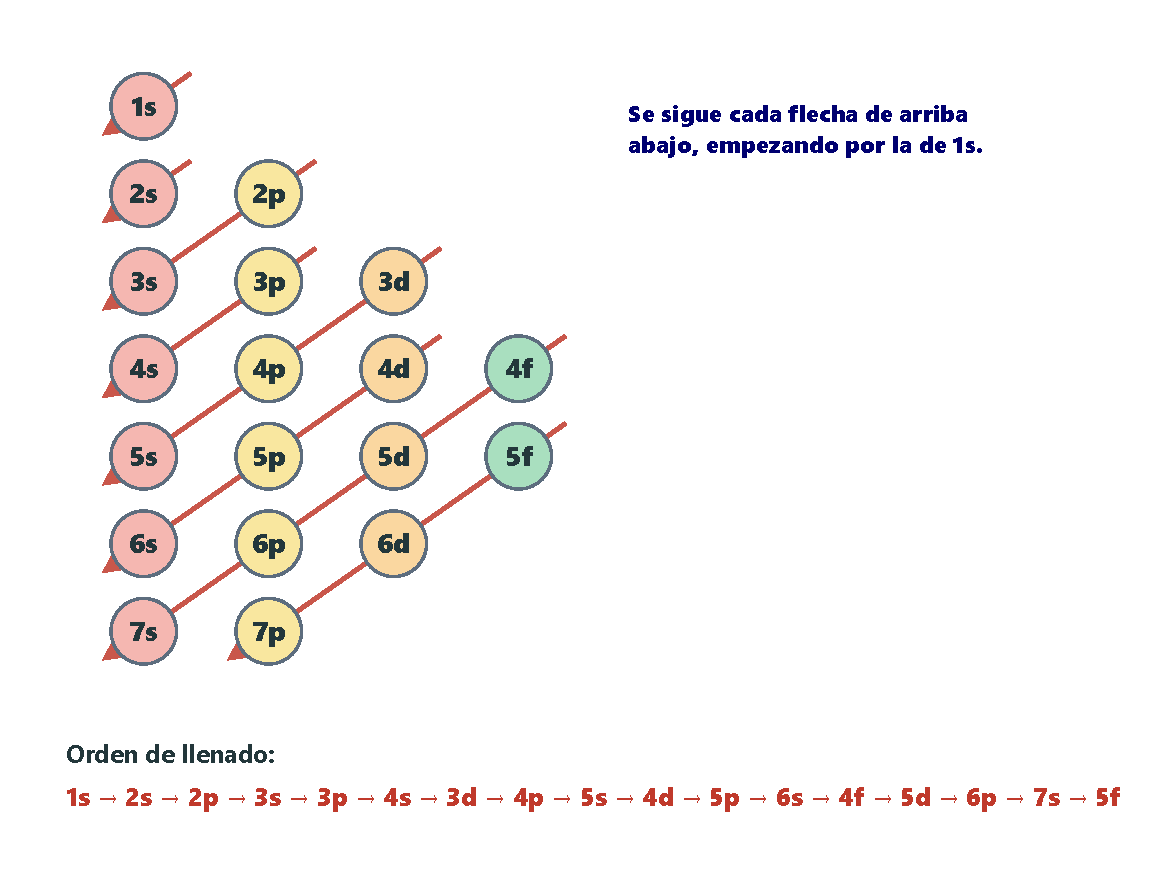
\includegraphics[width=0.7\textwidth]{images/UD2/diagrama_moeller}
    \caption{Diagrama de Moeller: orden de llenado de los subniveles.}
    \label{fig:moeller}
\end{figure}

\begin{example}
    \textbf{Configuración electrónica del sodio.} El sodio tiene \(Z = 11\), es decir, 11 electrones. Llenamos en orden: 2 en el 1s, 2 en el 2s, 6 en el 2p y el que queda en el 3s:
    \begin{centeredequation*}
        \ch{Na}:\ \mathrm{1s^2~2s^2~2p^6~3s^1}
    \end{centeredequation*}
    El exponente indica el número de electrones de cada subnivel; la suma de exponentes debe ser igual al número de electrones (\(2 + 2 + 6 + 1 = 11\)).
\end{example}

\begin{figure}[H]
    \centering
    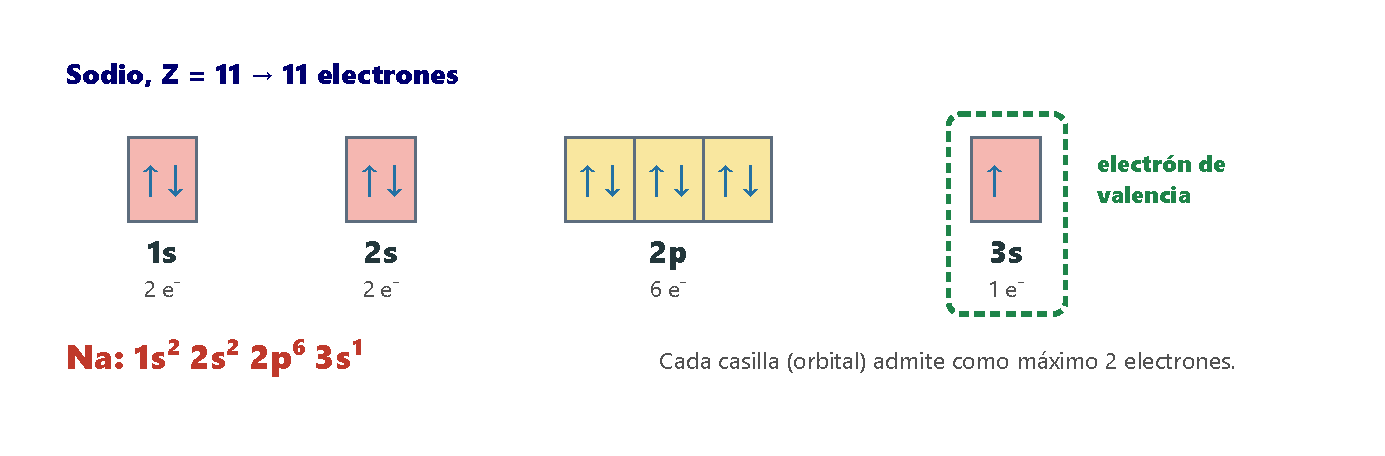
\includegraphics[width=0.75\textwidth]{images/UD2/configuracion_sodio}
    \caption{Diagrama de casillas de la configuración electrónica del sodio.}
    \label{fig:config_sodio}
\end{figure}

\begin{definition}[Electrones de valencia]
    Son los electrones del \textbf{último nivel} de energía ocupado. Por ejemplo, el sodio tiene \textbf{un} electrón de valencia (el del 3s). Son los responsables del comportamiento químico del elemento.
\end{definition}

\begin{remark}
    Para escribir configuraciones largas se puede abreviar usando el \textbf{gas noble} anterior entre corchetes. Por ejemplo, como el neón es \conf{1s^2~2s^2~2p^6}, el sodio queda \conf{[Ne]~3s^1}.
\end{remark}

\begin{exercise}
    ¿Qué cambios introduce el modelo de Bohr respecto al de Rutherford para poder explicar los espectros de rayas, en especial el del hidrógeno?
    \begin{solu}
        Introduce tres postulados: (1) existen órbitas circulares estables en las que el electrón gira sin emitir energía; (2) en cada órbita el electrón tiene una energía determinada, mayor cuanto más alejada está del núcleo; (3) el electrón solo emite (o absorbe) energía al saltar de un nivel a otro, y la energía emitida es la diferencia entre los niveles. Como solo hay ciertos saltos posibles, el espectro es de rayas.
    \end{solu}
\end{exercise}

\begin{exercise}
    Si el electrón no emite energía mientras gira en una órbita estable:
    \begin{enumerate}[label=\alph*)]
        \item ¿Cómo se originan las rayas de los espectros?
        \item ¿Cuándo puede emitir energía un electrón?
    \end{enumerate}
    \begin{solu}
        \begin{enumerate}[label=\alph*)]
            \item Las rayas de emisión se producen cuando un electrón pasa de un nivel superior a otro inferior; las de absorción, cuando pasa de un nivel inferior a otro superior absorbiendo energía.
            \item Solo cuando salta desde un nivel de energía superior a otro inferior.
        \end{enumerate}
    \end{solu}
\end{exercise}

\begin{exercise}
    Representa en tu cuaderno los saltos de energía posibles (hacia niveles inferiores) de un electrón que se encuentra en:
    \begin{enumerate}[label=\alph*)]
        \item El subnivel 3s.
        \item El subnivel 3p.
        \item El subnivel 2p.
    \end{enumerate}
    \begin{solu}
        \begin{enumerate}[label=\alph*)]
            \item Desde el 3s hay \textcolor{red}{tres} saltos posibles: a 2p, a 2s y a 1s.
            \item Desde el 3p hay \textcolor{red}{cuatro} saltos posibles: a 3s, a 2p, a 2s y a 1s.
            \item Desde el 2p hay \textcolor{red}{dos} saltos posibles: a 2s y a 1s.
        \end{enumerate}
    \end{solu}
\end{exercise}

\begin{exercise}
    Escribe la configuración electrónica de estos elementos:
    \begin{multicols}{4}
        \begin{enumerate}[label=\alph*)]
            \item H, \(Z = 1\)
            \item He, \(Z = 2\)
            \item Li, \(Z = 3\)
            \item B, \(Z = 5\)
            \item C, \(Z = 6\)
            \item N, \(Z = 7\)
            \item F, \(Z = 9\)
            \item Ne, \(Z = 10\)
        \end{enumerate}
    \end{multicols}
    \begin{solu}
        \begin{multicols}{2}
            \begin{enumerate}[label=\alph*)]
                \item H: \conf{1s^1}
                \item He: \conf{1s^2}
                \item Li: \conf{1s^2~2s^1}
                \item B: \conf{1s^2~2s^2~2p^1}
                \item C: \conf{1s^2~2s^2~2p^2}
                \item N: \conf{1s^2~2s^2~2p^3}
                \item F: \conf{1s^2~2s^2~2p^5}
                \item Ne: \conf{1s^2~2s^2~2p^6}
            \end{enumerate}
        \end{multicols}
    \end{solu}
\end{exercise}

\begin{exercise}
    Uno de los problemas del modelo de Rutherford era que el electrón, al ser una carga acelerada, debería emitir energía sin parar, lo que es incompatible con los espectros de rayas y con la estabilidad del átomo. ¿Qué postulado de Bohr soluciona este problema y cómo?
    \begin{solu}
        El primero: Bohr afirma que existen órbitas estables en las que el electrón gira a gran velocidad \textbf{sin emitir energía}. Así el electrón no pierde energía ni cae al núcleo.
    \end{solu}
\end{exercise}

\begin{exercise}
    Indica qué afirmaciones son verdaderas y corrige las falsas:
    \begin{enumerate}[label=\alph*)]
        \item El electrón gira muy rápido en una órbita estable en la que no emite energía.
        \item La energía del electrón en una órbita es menor cuanto más lejos del núcleo esté.
        \item Un electrón emite energía solo al pasar de un nivel superior a otro inferior.
        \item Cada elemento tiene un espectro de emisión característico.
        \item El subnivel 3d se llena justo después del 3p.
        \item El subnivel 4p se llena justo después del 4s.
    \end{enumerate}
    \begin{solu}
        \begin{enumerate}[label=\alph*)]
            \item Verdadera.
            \item \textcolor{red}{Falsa.} La energía es \textbf{mayor} cuanto más alejada del núcleo está la órbita.
            \item Verdadera.
            \item Verdadera.
            \item \textcolor{red}{Falsa.} Después del 3p se llena el 4s, y después el 3d.
            \item \textcolor{red}{Falsa.} Después del 4s se llena el 3d, y después el 4p.
        \end{enumerate}
    \end{solu}
\end{exercise}

\begin{exercise}
    Dibuja los dos primeros niveles de energía con sus subniveles. Coloca un electrón en el subnivel de mayor energía y razona cuántas rayas distintas podrían aparecer en el espectro cuando ese electrón vuelva a niveles inferiores.
    \begin{solu}
        Los subniveles son 1s, 2s y 2p (de menor a mayor energía). Un electrón en el 2p puede saltar al 2s o al 1s: aparecerían \textcolor{red}{dos rayas} diferentes. (Si después baja del 2s al 1s se produciría una tercera raya.)
    \end{solu}
\end{exercise}

\begin{exercise}
    ¿En qué subnivel tiene más energía un electrón: en el 2s o en el 3p?
    \begin{solu}
        En el \textcolor{red}{3p}, que pertenece a un nivel superior y se llena después del 2s.
    \end{solu}
\end{exercise}

\begin{exercise}
    Escribe la configuración electrónica de los siguientes átomos y, cuando se indique, de sus iones:
    \begin{multicols}{2}
        \begin{enumerate}[label=\alph*)]
            \item Aluminio (\(Z = 13\)) y \ch{Al^{3+}}
            \item Cloro (\(Z = 17\)) y \ch{Cl-}
            \item Calcio (\(Z = 20\)) y \ch{Ca^{2+}}
            \item Zinc (\(Z = 30\))
            \item Criptón (\(Z = 36\))
            \item Bario (\(Z = 56\)) y \ch{Ba^{2+}}
            \item Polonio (\(Z = 84\))
            \item Lantano (\(Z = 57\))
        \end{enumerate}
    \end{multicols}
    \begin{solu}
        \begin{enumerate}[label=\alph*)]
            \item Al: \conf{1s^2~2s^2~2p^6~3s^2~3p^1}; \quad \ch{Al^{3+}}: \conf{1s^2~2s^2~2p^6}
            \item Cl: \conf{1s^2~2s^2~2p^6~3s^2~3p^5}; \quad \ch{Cl-}: \conf{1s^2~2s^2~2p^6~3s^2~3p^6}
            \item Ca: \conf{1s^2~2s^2~2p^6~3s^2~3p^6~4s^2}; \quad \ch{Ca^{2+}}: \conf{1s^2~2s^2~2p^6~3s^2~3p^6}
            \item Zn: \conf{1s^2~2s^2~2p^6~3s^2~3p^6~4s^2~3d^{10}}
            \item Kr: \conf{1s^2~2s^2~2p^6~3s^2~3p^6~4s^2~3d^{10}~4p^6}
            \item Ba: \conf{[Kr]~5s^2~4d^{10}~5p^6~6s^2}; \quad \ch{Ba^{2+}}: \conf{[Kr]~5s^2~4d^{10}~5p^6}
            \item Po: \conf{[Kr]~5s^2~4d^{10}~5p^6~6s^2~4f^{14}~5d^{10}~6p^4}
            \item La: \conf{[Kr]~5s^2~4d^{10}~5p^6~6s^2~5d^1} (el lantano es una excepción: su último electrón entra en el 5d y no en el 4f).
        \end{enumerate}
    \end{solu}
\end{exercise}

%========================================================================================
\section{¿Cómo se clasifican los elementos químicos? La tabla periódica}
%========================================================================================

Una de las primeras clasificaciones de los elementos los dividía en \textbf{metales} y \textbf{no metales}, según sus propiedades:

\begin{table}[H]
    \centering
    % --- tabla antigua ---
    % \begin{tblr}{colspec={X[l]X[l]}, hlines, vlines, row{1}={bg=ocre!85, fg=white, font=\bfseries, halign=c}}
        % Metales & No metales \\
        % {\textbullet~Tienen brillo metálico.\\ \textbullet~Conducen bien el calor y la electricidad.\\ \textbullet~Son dúctiles (forman hilos) y maleables (forman láminas).\\ \textbullet~Son sólidos a temperatura ambiente, salvo el mercurio.}
        % & {\textbullet~No tienen brillo metálico.\\ \textbullet~Conducen mal el calor y la electricidad.\\ \textbullet~A temperatura ambiente pueden ser sólidos, líquidos o gases.\\ \textbullet~Suelen tener puntos de fusión bajos.} \\
    % \end{tblr}
    % --- tabla nueva ---
    \begin{tabular}{@{}L{0.45\linewidth} L{0.45\linewidth}@{}}
        \toprule
        \textbf{Metales} & \textbf{No metales} \\
        \midrule
        \textbullet~Tienen brillo metálico.\newline \textbullet~Conducen bien el calor y la electricidad.\newline \textbullet~Son dúctiles (forman hilos) y maleables (forman láminas).\newline \textbullet~Son sólidos a temperatura ambiente, salvo el mercurio. & \textbullet~No tienen brillo metálico.\newline \textbullet~Conducen mal el calor y la electricidad.\newline \textbullet~A temperatura ambiente pueden ser sólidos, líquidos o gases.\newline \textbullet~Suelen tener puntos de fusión bajos. \\
        \bottomrule
    \end{tabular}
    \caption{Propiedades generales de metales y no metales.}
    \label{tab:metales}
\end{table}

\subsection{La tabla periódica actual}

Hoy los elementos se organizan en el \textbf{sistema periódico}, ordenados de izquierda a derecha y de arriba abajo por \textbf{número atómico creciente}. La posición de cada elemento depende, por tanto, de su número de protones y, en consecuencia, de su número de electrones.

Los 118 elementos conocidos se reparten en \textbf{18 columnas o grupos} y \textbf{7 filas o períodos}:

\begin{itemize}
    \item \negsubro{Grupos.} Los elementos de una misma columna tienen el \textbf{mismo número de electrones en su último nivel} (electrones de valencia) y, por eso, \textbf{propiedades químicas parecidas}. Se numeran del 1 al 18.
    \item \negsubro{Períodos.} Los elementos de una misma fila tienen el \textbf{mismo número de niveles electrónicos} ocupados, y sus propiedades cambian poco a poco a lo largo de la fila. Se numeran del 1 al 7.
    \begin{itemize}
        \item Períodos \textbf{cortos}: el 1 (2 elementos), el 2 y el 3 (8 elementos cada uno).
        \item Períodos \textbf{largos}: el 4 y el 5 (18 elementos cada uno).
        \item Períodos \textbf{muy largos}: el 6 y el 7 (32 elementos cada uno), que incluyen los lantanoides y actinoides, colocados aparte en dos filas bajo la tabla.
    \end{itemize}
\end{itemize}

\begin{figure}[H]
    \centering
    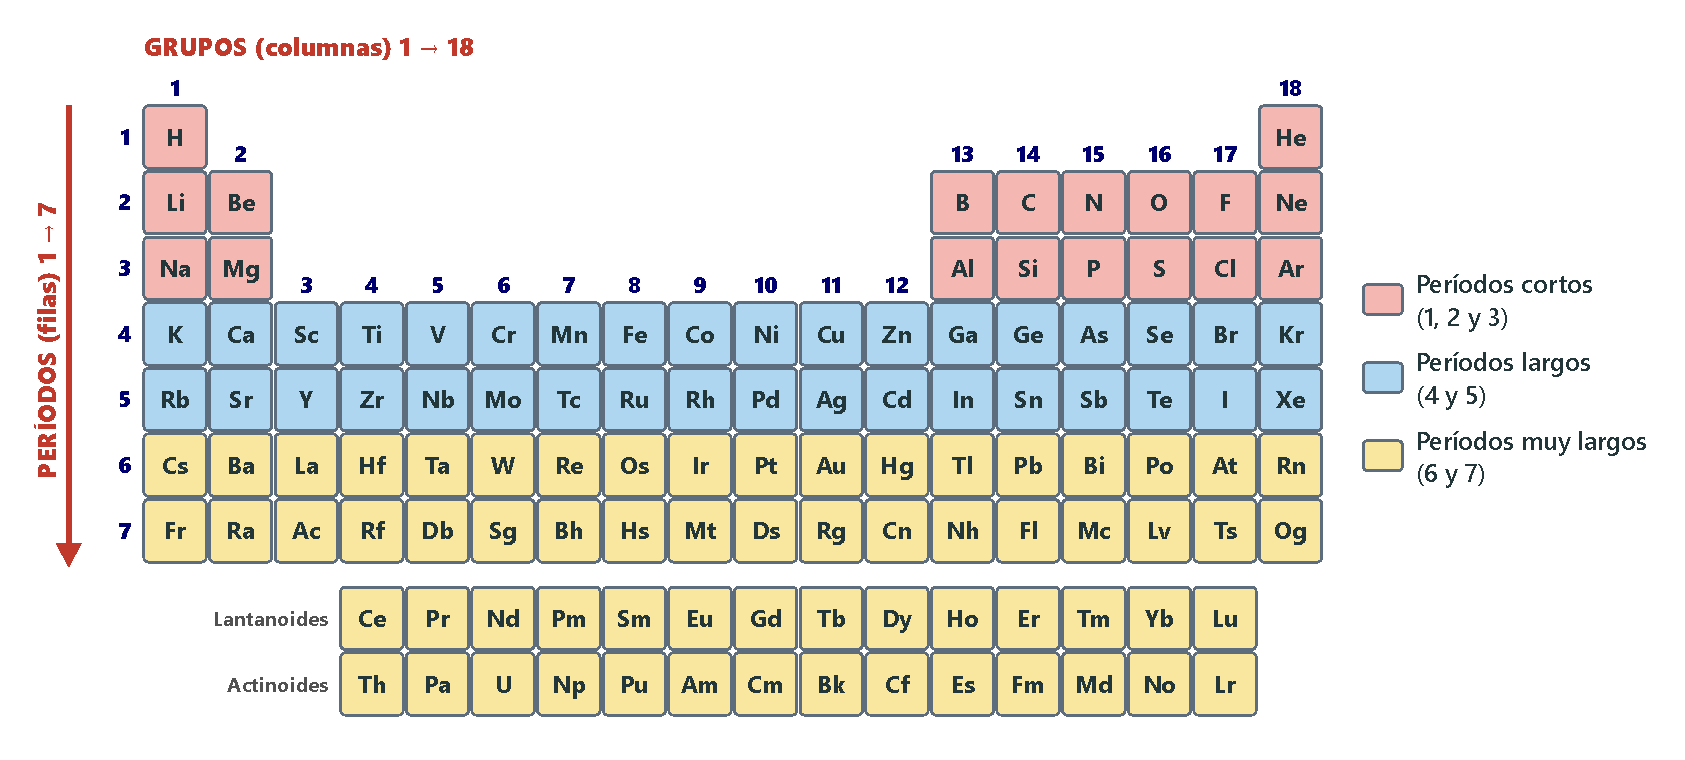
\includegraphics[width=0.9\textwidth]{images/UD2/grupos_periodos}
    \caption{Grupos y períodos de la tabla periódica.}
    \label{fig:grupos_periodos}
\end{figure}

\begin{sidewaysfigure}
    \centering
    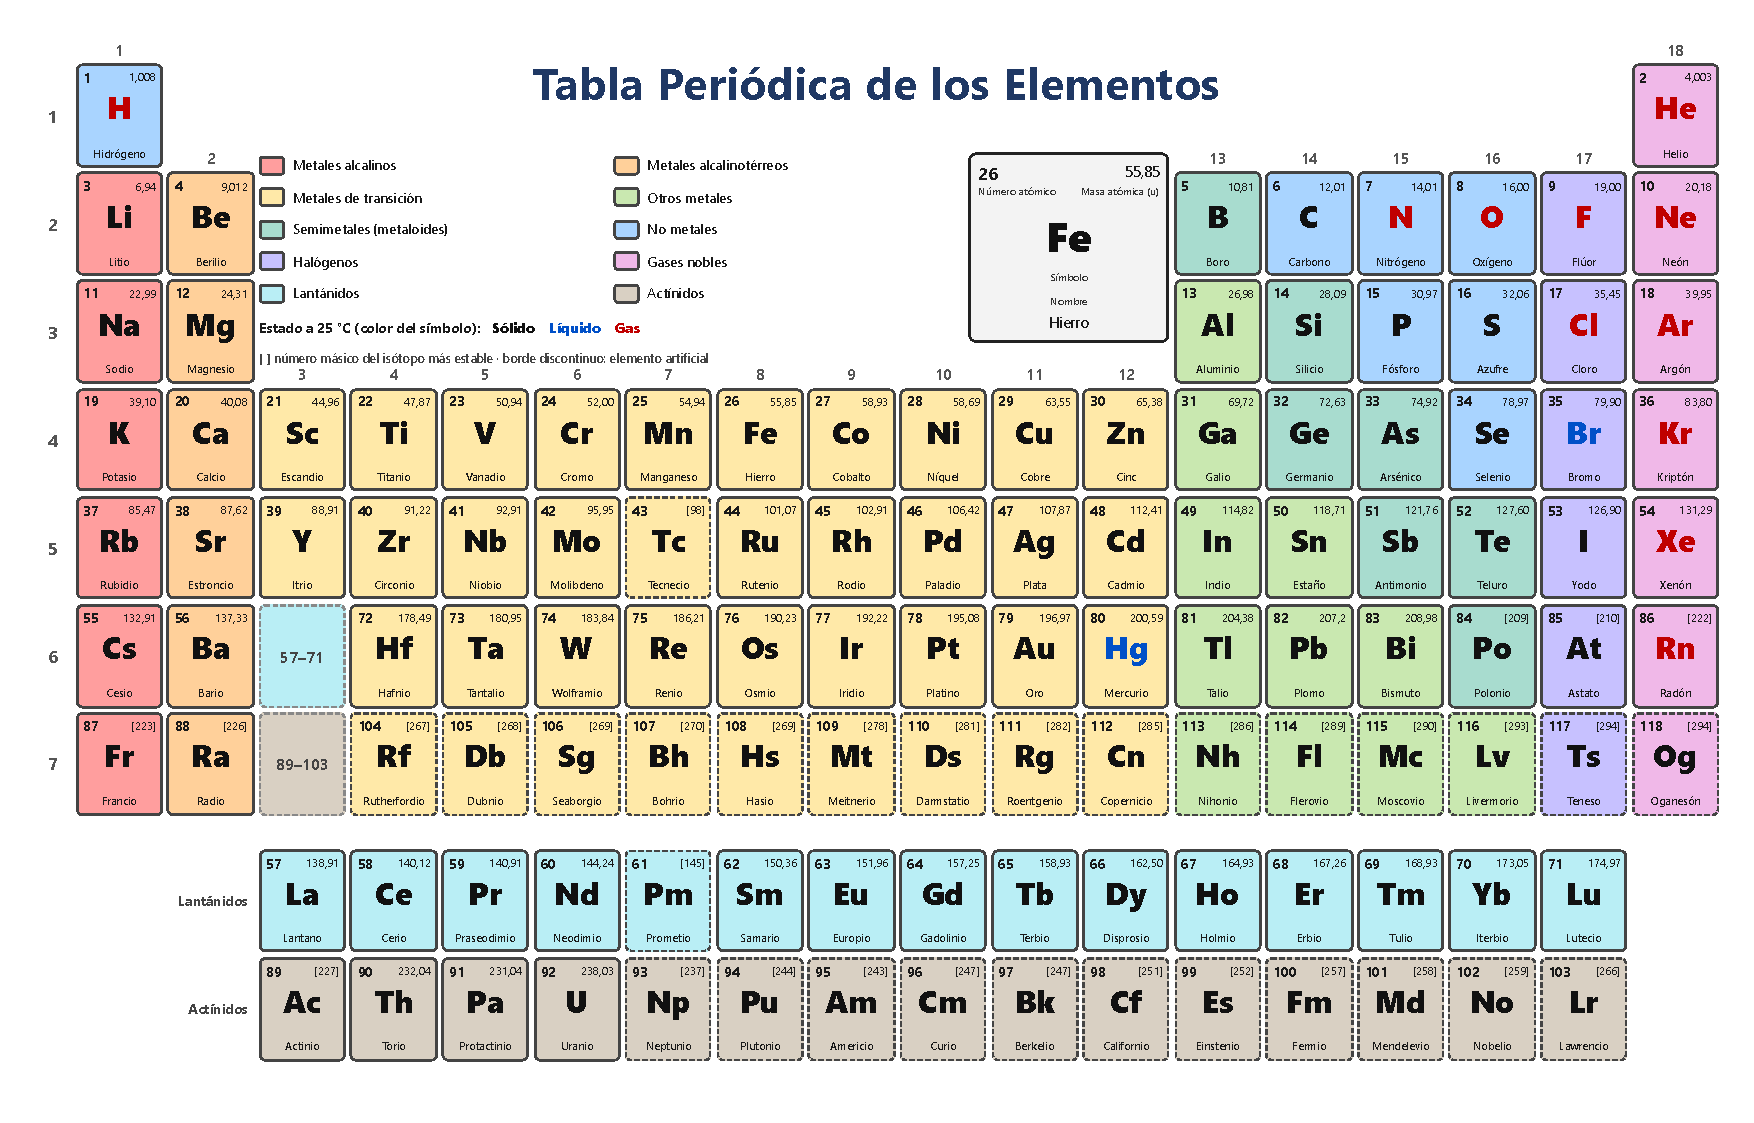
\includegraphics[width=\linewidth,height=0.9\textheight,keepaspectratio]{images/UD2/tabla_periodica}
    \caption{Tabla periódica de los elementos.}
    \label{fig:tabla_periodica}
\end{sidewaysfigure}

\subsection{Regularidades de los elementos en la tabla}

Al ordenar los elementos por número atómico, muchas propiedades se repiten periódicamente.

\paragraph{A lo largo de un período} (de izquierda a derecha):
\begin{itemize}
    \item El número de electrones externos aumenta de uno en uno. El electrón que diferencia a un elemento del anterior se llama \textbf{electrón diferenciador}.
    \item La masa atómica aumenta, salvo alguna excepción.
    \item El carácter metálico disminuye: los metales están a la izquierda y los no metales a la derecha.
    \item Los puntos de fusión y ebullición aumentan hasta la mitad del período y luego disminuyen.
\end{itemize}

\paragraph{Al bajar en un grupo:}
\begin{itemize}
    \item El número de electrones del último nivel es el mismo, por eso las propiedades son similares.
    \item La masa atómica aumenta.
    \item El carácter metálico aumenta.
    \item Los puntos de fusión y ebullición varían ligeramente.
\end{itemize}

\begin{figure}[H]
    \centering
    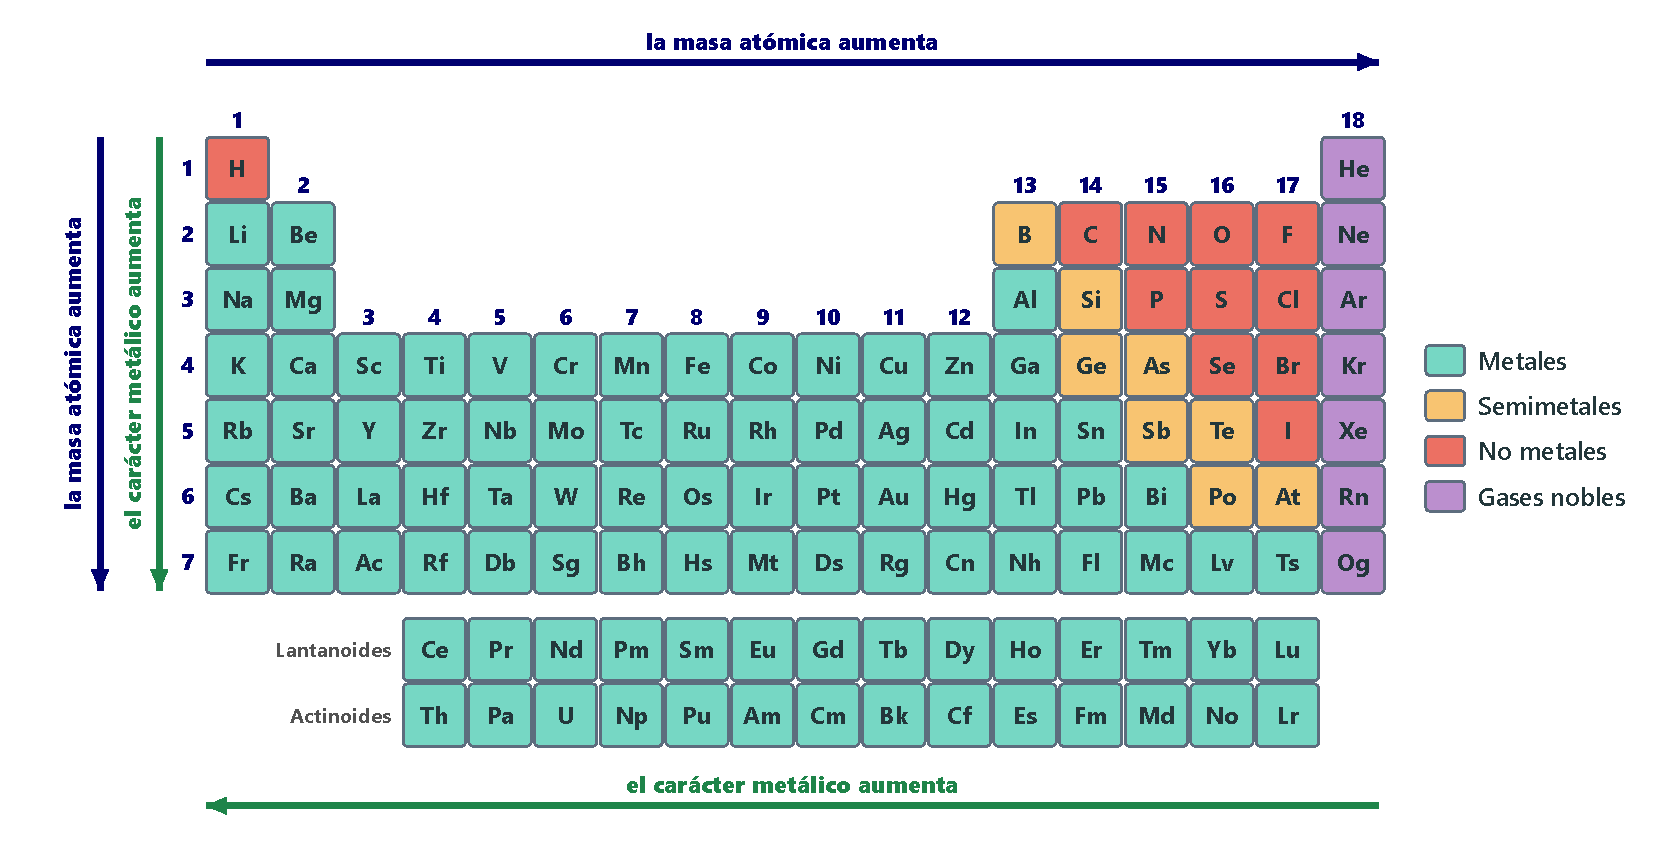
\includegraphics[width=0.95\textwidth]{images/UD2/regularidades}
    \caption{Metales, semimetales, no metales y gases nobles, y variación de la masa atómica y del carácter metálico.}
    \label{fig:regularidades}
\end{figure}

\begin{table}[H]
    \centering
    % --- tabla antigua ---
    % \begin{tblr}{colspec={lll}, row{1}={bg=ocre!85, fg=white, font=\bfseries}, hlines}
        % Grupos 1 a 6 & Grupos 7 a 12 & Grupos 13 a 18 \\
        % 1. Alcalinos & 7. Familia del manganeso & 13. Térreos (familia del boro) \\
        % 2. Alcalinotérreos & 8. Familia del hierro & 14. Carbonoideos \\
        % 3. Familia del escandio & 9. Familia del cobalto & 15. Nitrogenoideos \\
        % 4. Familia del titanio & 10. Familia del níquel & 16. Anfígenos \\
        % 5. Familia del vanadio & 11. Familia del cobre & 17. Halógenos \\
        % 6. Familia del cromo & 12. Familia del zinc & 18. Gases nobles \\
    % \end{tblr}
    % --- tabla nueva ---
    \begin{tabular}{@{}lll@{}}
        \toprule
        \textbf{Grupos 1 a 6} & \textbf{Grupos 7 a 12} & \textbf{Grupos 13 a 18} \\
        \midrule
        1. Alcalinos & 7. Familia del manganeso & 13. Térreos (familia del boro) \\[3pt]
        2. Alcalinotérreos & 8. Familia del hierro & 14. Carbonoideos \\[3pt]
        3. Familia del escandio & 9. Familia del cobalto & 15. Nitrogenoideos \\[3pt]
        4. Familia del titanio & 10. Familia del níquel & 16. Anfígenos \\[3pt]
        5. Familia del vanadio & 11. Familia del cobre & 17. Halógenos \\[3pt]
        6. Familia del cromo & 12. Familia del zinc & 18. Gases nobles \\
        \bottomrule
    \end{tabular}
    \caption{Nombres de los grupos de la tabla periódica.}
    \label{tab:nombres_grupos}
\end{table}

\subsection{Configuración electrónica y posición en la tabla}

La tabla periódica es, en realidad, un mapa de las configuraciones electrónicas. Veamos cómo se van llenando los subniveles período a período:

\begin{itemize}
    \item \negsubro{Período 1.} El hidrógeno (\conf{1s^1}) y el helio (\conf{1s^2}) llenan el subnivel 1s, que solo admite dos electrones.
    \item \negsubro{Período 2.} Del litio (\conf{1s^2~2s^1}) al neón se llenan el 2s y el 2p: \(2 + 6 = 8\) electrones, 8 elementos.
    \item \negsubro{Período 3.} Se repite el proceso con el 3s y el 3p, del sodio (\conf{[Ne]~3s^1}) al argón (\conf{[Ne]~3s^2~3p^6}).
    \item \negsubro{Período 4.} El potasio y el calcio colocan sus electrones en el 4s (que tiene menos energía que el 3d). Desde el escandio hasta el zinc se llena el 3d (10 elementos) y, después, el 4p, hasta el criptón: 18 elementos.
    \item \negsubro{Período 5.} Se llenan el 5s (Rb y Sr), el 4d (del Y al Cd) y el 5p (del In al Xe): 18 elementos.
    \item \negsubro{Período 6.} El cesio y el bario llenan el 6s. El lantano coloca un electrón en el 5d, pero a partir del cerio se llena el \textbf{4f} (14 elementos, los \textbf{lantanoides}). Después se completa el 5d (del Hf al Hg) y el 6p (del Tl al Rn).
    \item \negsubro{Período 7.} Ocurre algo análogo: 7s, un electrón en el 6d (actinio), el \textbf{5f} desde el torio (los \textbf{actinoides}), y después el 6d y el 7p.
\end{itemize}

\begin{figure}[H]
    \centering
    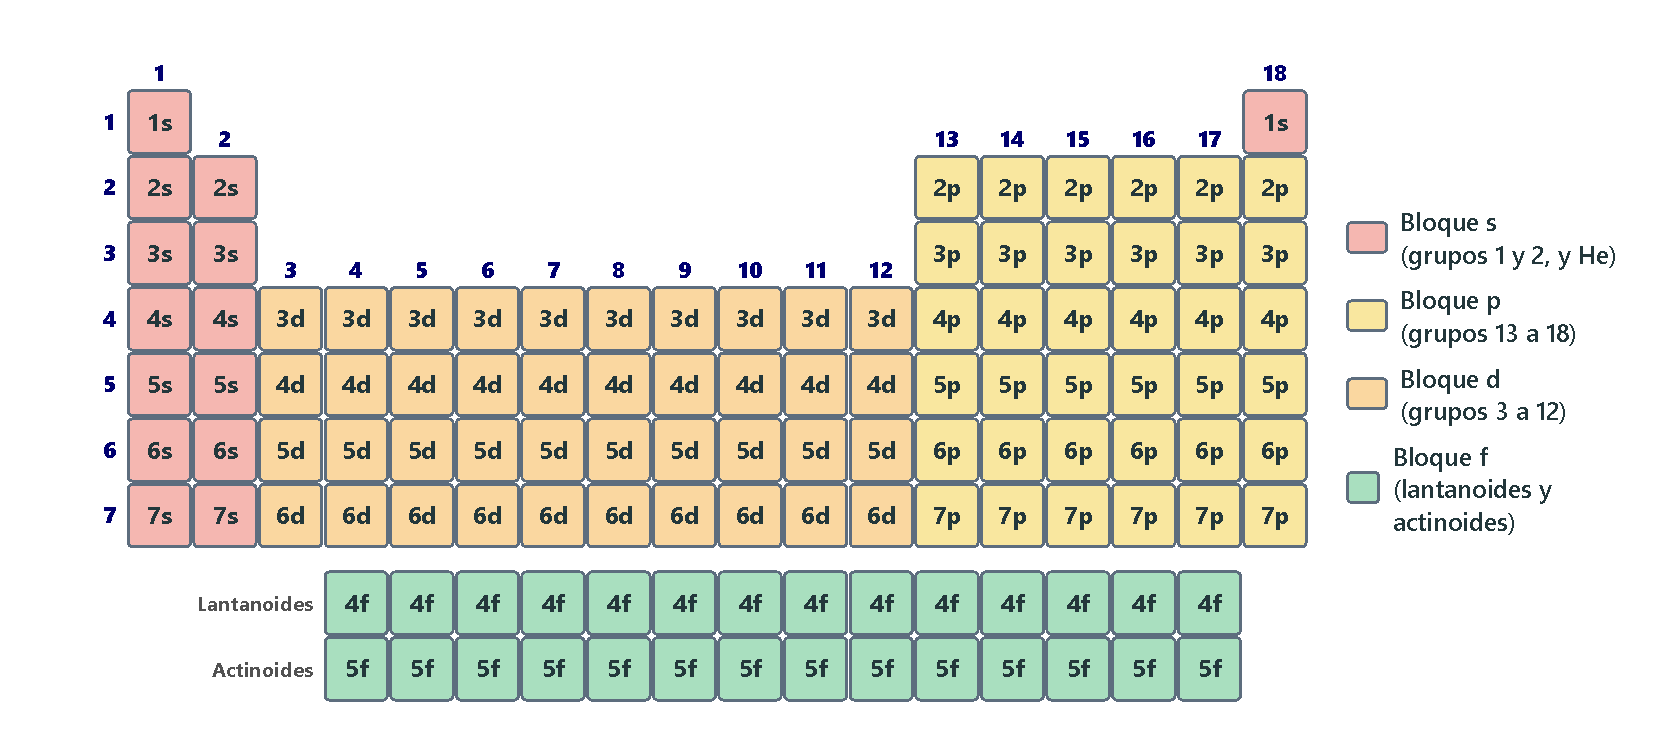
\includegraphics[width=0.9\textwidth]{images/UD2/bloques_spdf}
    \caption{Subnivel que ocupa el electrón diferenciador en cada zona de la tabla: bloques s, p, d y f.}
    \label{fig:bloques}
\end{figure}

\begin{remark}
    \textbf{Truco para leer la tabla:} el número del \textbf{período} coincide con el último nivel ocupado (el número más alto de la configuración), y en los elementos de los bloques s y p los \textbf{electrones de valencia} se deducen del grupo: 1 en el grupo 1, 2 en el grupo 2, y \(\text{grupo} - 10\) en los grupos 13 a 18 (salvo el helio, que tiene 2).
\end{remark}

\begin{exercise}
    Escribe el nombre de cinco elementos metálicos y de cinco no metálicos.
    \begin{solu}
        Respuesta libre. Por ejemplo, metales: hierro, cobre, sodio, aluminio, oro. No metales: oxígeno, nitrógeno, carbono, azufre, cloro.
    \end{solu}
\end{exercise}

\begin{exercise}
    Nombra tres elementos situados en:
    \begin{multicols}{2}
        \begin{enumerate}[label=\alph*)]
            \item Un período corto.
            \item Un período largo.
            \item Un período muy largo.
            \item El grupo 18.
            \item El período 5.
        \end{enumerate}
    \end{multicols}
    \begin{solu}
        Respuesta libre. Por ejemplo: a) sodio, aluminio, fósforo; b) hierro, cadmio, indio; c) cesio, osmio, oro; d) helio, neón, argón; e) itrio, plata, yodo.
    \end{solu}
\end{exercise}

\begin{exercise}
    Indica el grupo y el período de cada uno de estos elementos: fósforo, bromo, estroncio, rutenio, xenón, cesio, mercurio, lantano y actinio.
    \begin{solu}
        Fósforo: grupo 15, período 3. Bromo: grupo 17, período 4. Estroncio: grupo 2, período 5. Rutenio: grupo 8, período 5. Xenón: grupo 18, período 5. Cesio: grupo 1, período 6. Mercurio: grupo 12, período 6. Lantano: grupo 3, período 6. Actinio: grupo 3, período 7.
    \end{solu}
\end{exercise}

\begin{exercise}
    ¿Cuáles de estos elementos tienen el mismo número de electrones de valencia? Litio, calcio, cloro, rubidio, neón, sodio, hierro, cesio, plomo, potasio.
    \begin{solu}
        Litio, rubidio, sodio, cesio y potasio: todos son del grupo 1 y tienen \textcolor{red}{un electrón de valencia}.
    \end{solu}
\end{exercise}

\begin{exercise}
    En cada pareja, ¿cuál tiene mayor carácter metálico?
    \begin{multicols}{4}
        \begin{enumerate}[label=\alph*)]
            \item Be / Ba
            \item F / I
            \item Sc / Zn
            \item C / Pb
            \item Cu / Au
            \item Li / Cs
            \item Pd / I
            \item B / In
        \end{enumerate}
    \end{multicols}
    \begin{solu}
        \textcolor{blue}{El carácter metálico aumenta hacia abajo en un grupo y hacia la izquierda en un período.}
        a) Ba; b) I; c) Sc; d) Pb; e) Au; f) Cs; g) Pd; h) In.
    \end{solu}
\end{exercise}

\begin{exercise}
    Nombra cinco elementos con el mismo número de niveles electrónicos que el azufre (\(Z = 16\)).
    \begin{solu}
        El azufre está en el período 3, así que tiene 3 niveles. Por ejemplo: sodio, magnesio, aluminio, silicio y fósforo (también cloro y argón).
    \end{solu}
\end{exercise}

\begin{exercise}
    Indica a qué familia pertenece cada elemento: cloro, cesio, silicio, fósforo, magnesio, argón.
    \begin{solu}
        Cloro: halógenos. Cesio: alcalinos. Silicio: carbonoideos. Fósforo: nitrogenoideos. Magnesio: alcalinotérreos. Argón: gases nobles.
    \end{solu}
\end{exercise}

\begin{exercise}
    Nombra cinco elementos con el mismo número de electrones en el último nivel que el aluminio (\(Z = 13\)).
    \begin{solu}
        Los del grupo 13: boro, galio, indio, talio y nihonio.
    \end{solu}
\end{exercise}

\begin{exercise}
    ¿Cuántos niveles electrónicos tienen los átomos que van del litio al neón? ¿Y los que van del sodio al argón?
    \begin{solu}
        Del litio al neón (período 2): \textcolor{red}{dos niveles}. Del sodio al argón (período 3): \textcolor{red}{tres niveles}.
    \end{solu}
\end{exercise}

\begin{exercise}
    ¿Cómo cambia el número de electrones del último nivel al pasar de un elemento al siguiente dentro de un período?
    \begin{solu}
        Aumenta de uno en uno (el electrón diferenciador).
    \end{solu}
\end{exercise}

\begin{exercise}
    El electrón diferenciador es el que distingue a un elemento del anterior. Indica en qué subnivel se encuentra el electrón diferenciador de: litio, neón, magnesio, escandio, bromo, rubidio, circonio, yodo, lantano, cerio, actinio y torio.
    \begin{solu}
        Litio: 2s. Neón: 2p. Magnesio: 3s. Escandio: 3d. Bromo: 4p. Rubidio: 5s. Circonio: 4d. Yodo: 5p. Lantano: 5d. Cerio: 4f. Actinio: 6d. Torio: 5f.
    \end{solu}
\end{exercise}

\begin{exercise}
    ¿Qué elemento es más metálico, el sodio o el cesio? ¿Y cuál es más no metálico, el carbono o el flúor?
    \begin{solu}
        El \textcolor{red}{cesio} es más metálico (está más abajo en el grupo 1). El \textcolor{red}{flúor} es más no metálico (está más a la derecha en el período 2).
    \end{solu}
\end{exercise}

\begin{exercise}
    Escribe el nombre, el símbolo y el número atómico de tres elementos que:
    \begin{enumerate}[label=\alph*)]
        \item Tengan el mismo número de niveles que el silicio.
        \item Tengan sus electrones repartidos en cuatro niveles.
        \item Pertenezcan a un período corto.
    \end{enumerate}
    \begin{solu}
        Respuesta libre. Por ejemplo: a) sodio, Na, 11; azufre, S, 16; cloro, Cl, 17. b) Cualquiera del período 4: potasio, K, 19; hierro, Fe, 26; bromo, Br, 35. c) Cualquiera de los períodos 1, 2 o 3: helio, He, 2; carbono, C, 6; magnesio, Mg, 12.
    \end{solu}
\end{exercise}

\begin{exercise}
    Escribe la configuración electrónica de los gases nobles. ¿Qué tienen todos en común?
    \begin{solu}
        He: \conf{1s^2}\\
        Ne: \conf{1s^2~2s^2~2p^6}\\
        Ar: \conf{1s^2~2s^2~2p^6~3s^2~3p^6}\\
        Kr: \conf{[Ar]~4s^2~3d^{10}~4p^6}\\
        Xe: \conf{[Kr]~5s^2~4d^{10}~5p^6}\\
        Rn: \conf{[Xe]~6s^2~4f^{14}~5d^{10}~6p^6}\\
        Todos tienen su último nivel completo: 8 electrones (\conf{ns^2~np^6}), salvo el helio, que tiene 2.
    \end{solu}
\end{exercise}

\begin{exercise}
    Explica por qué la configuración electrónica del ion \ch{Na+} es \conf{1s^2~2s^2~2p^6}.
    \begin{solu}
        El sodio neutro es \conf{1s^2~2s^2~2p^6~3s^1}. Al perder su electrón de valencia (el del 3s) se forma \ch{Na+}, que queda con \conf{1s^2~2s^2~2p^6}, la misma configuración que el neón.
    \end{solu}
\end{exercise}

\begin{exercise}
    Explica por qué la configuración del ion \ch{Cl-} es \conf{1s^2~2s^2~2p^6~3s^2~3p^6}.
    \begin{solu}
        El cloro neutro es \conf{1s^2~2s^2~2p^6~3s^2~3p^5}. Al ganar un electrón, este entra en el 3p, que queda completo con 6 electrones: es la configuración del argón.
    \end{solu}
\end{exercise}

\begin{exercise}
    ¿A qué elemento corresponde la configuración \conf{1s^2~2s^2~2p^6~3s^2~3p^3}?
    \begin{solu}
        \textcolor{blue}{Sumamos los electrones: \(2 + 2 + 6 + 2 + 3 = 15\).} Es el \textcolor{red}{fósforo, \(Z = 15\)}.
    \end{solu}
\end{exercise}

\begin{exercise}
    Dibuja el contorno de la tabla periódica en tu cuaderno y señala el grupo de los alcalinotérreos. Después escribe:
    \begin{enumerate}[label=\alph*)]
        \item La configuración de su último nivel.
        \item La configuración de sus iones cuando pierden dos electrones.
    \end{enumerate}
    \begin{solu}
        \begin{enumerate}[label=\alph*)]
            \item \conf{ns^2}, donde \(n\) es el número del período.
            \item Al perder los dos electrones del \conf{ns^2}, cada ion queda con la configuración del gas noble anterior (por ejemplo, \ch{Mg^{2+}}: \conf{1s^2~2s^2~2p^6}, como el neón).
        \end{enumerate}
    \end{solu}
\end{exercise}

\begin{exercise}
    Localiza el grupo 16 (anfígenos) y escribe la configuración electrónica de su último nivel.
    \begin{solu}
        \conf{ns^2~np^4}: tienen 6 electrones de valencia.
    \end{solu}
\end{exercise}

\begin{exercise}
    Sobre los elementos del grupo 18:
    \begin{enumerate}[label=\alph*)]
        \item ¿Cuántos electrones tienen en su último nivel?
        \item ¿Cuántos electrones caben como máximo en los subniveles s y p de ese último nivel?
    \end{enumerate}
    \begin{solu}
        a) 8 electrones (el helio, 2). b) 8 (2 en el s y 6 en el p): el último nivel está completo, por eso son muy estables.
    \end{solu}
\end{exercise}

\begin{exercise}
    Sobre los elementos del grupo 1:
    \begin{enumerate}[label=\alph*)]
        \item ¿Cuántos electrones tienen en su último nivel?
        \item ¿Cuántos tendrían que perder para quedarse con el último nivel completo?
        \item ¿Son metales o no metales?
        \item ¿Cómo se llama este grupo?
    \end{enumerate}
    \begin{solu}
        a) Un electrón (\conf{ns^1}). b) Uno: al perderlo quedan con la configuración del gas noble anterior. c) Son metales (excepto el hidrógeno). d) Alcalinos.
    \end{solu}
\end{exercise}

\begin{exercise}
    Sobre los elementos del grupo 15:
    \begin{enumerate}[label=\alph*)]
        \item ¿Cuántos electrones tienen en su último nivel?
        \item ¿Les conviene ganar o perder electrones para completar ese nivel? ¿Cuántos?
        \item ¿Son metales o no metales?
    \end{enumerate}
    \begin{solu}
        a) Cinco (\conf{ns^2~np^3}). b) Ganar tres electrones. c) El nitrógeno y el fósforo son no metales; el arsénico y el antimonio, semimetales; el bismuto, un metal.
    \end{solu}
\end{exercise}

\begin{exercise}
    Los elementos que forman parte de los seres vivos se llaman bioelementos. Investiga cuáles son, en qué proporción están en el cuerpo humano y qué funciones cumplen.
    \begin{solu}
        Respuesta libre. Los principales son C, H, O y N (más del \qty{95}{\percent} de la masa), junto con P y S. Otros, en menor cantidad: Ca (huesos), Na y K (impulso nervioso), Fe (hemoglobina), Mg, Cl, I (tiroides)\ldots
    \end{solu}
\end{exercise}

\begin{exercise}
    ¿Qué elemento es el primero en empezar a llenar cada uno de estos subniveles?
    \begin{multicols}{5}
        \begin{enumerate}[label=\alph*)]
            \item 3p
            \item 4s
            \item 4d
            \item 5d
            \item 4f
        \end{enumerate}
    \end{multicols}
    \begin{solu}
        a) Aluminio. b) Potasio. c) Itrio. d) Lantano. e) Cerio.
    \end{solu}
\end{exercise}

%========================================================================================
\section{Tipos de elementos químicos}
%========================================================================================

Según el subnivel en el que se aloja su electrón diferenciador, los elementos se clasifican en tres tipos: \textbf{representativos}, \textbf{de transición} y \textbf{de transición interna}.

\begin{figure}[H]
    \centering
    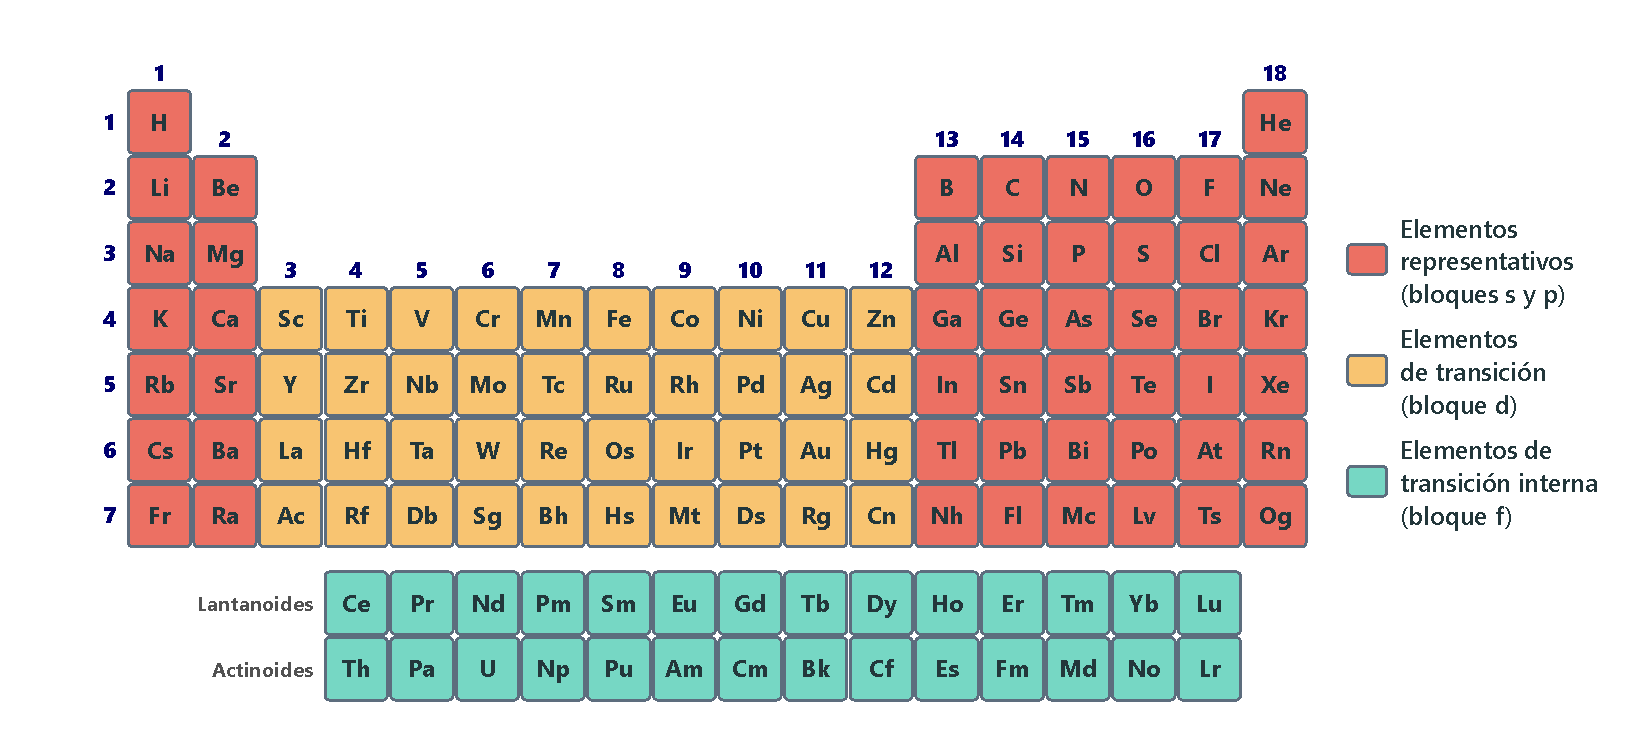
\includegraphics[width=0.9\textwidth]{images/UD2/tipos_elementos}
    \caption{Tipos de elementos según su configuración electrónica.}
    \label{fig:tipos_elementos}
\end{figure}

\subsection{Los elementos representativos}

Su configuración electrónica externa va desde \conf{ns^1} hasta \conf{ns^2~np^6}: solo ocupan los subniveles s y p del último nivel. Son los más abundantes en la Tierra y en el universo. Se distinguen tres bloques:

\begin{itemize}
    \item El \textbf{bloque s}: grupos 1 y 2.
    \item El \textbf{bloque p}: grupos 13 a 17.
    \item Los \textbf{gases nobles} (grupo 18), con configuración \conf{ns^2~np^6}, de máxima estabilidad.
\end{itemize}

\subsection{Metales, no metales y semimetales}

El hidrógeno y el helio, del primer período, son no metales. En el resto de períodos, los elementos representativos pasan de \textbf{metales} (a la izquierda) a \textbf{no metales} (a la derecha), pasando por los \textbf{semimetales}.

\begin{itemize}
    \item Los átomos \textbf{metálicos} tienen pocos electrones externos y los pierden con facilidad.
    \item Los \textbf{no metálicos} tienen más electrones en su última capa, más fuertemente retenidos; tienden a ganarlos.
    \item Los \textbf{semimetales} (B, Si, Ge, As, Sb, Te\ldots) tienen propiedades intermedias: por ejemplo, son \textbf{semiconductores}, por eso se usan en los chips electrónicos.
\end{itemize}

\subsection{Los elementos de transición}

Son aquellos cuyo último electrón entra en un subnivel \textbf{d}: forman el \textbf{bloque d}. Su configuración externa va de \conf{(n-1)d^1~ns^2} a \conf{(n-1)d^{10}~ns^2}. Ocupan la parte central de la tabla, los grupos 3 a 12 (diez grupos, uno por cada electrón d). Sus propiedades comunes son:

\begin{itemize}
    \item Todos son \textbf{metales}.
    \item Son sólidos, excepto el mercurio, que es líquido.
    \item Son duros y tienen puntos de fusión y ebullición elevados.
    \item Son muy buenos conductores del calor y de la electricidad.
    \item Sus compuestos suelen tener \textbf{colores} llamativos.
\end{itemize}

\subsection{Los elementos de transición interna}

Al llenarse los subniveles \textbf{4f} y \textbf{5f} aparecen dos series de catorce elementos, el \textbf{bloque f}, que se sitúan en las dos filas separadas de la parte inferior de la tabla. Sus propiedades se parecen a las de los metales de transición.

\begin{itemize}
    \item \negsubro{Lantanoides.} Del cerio (\(Z = 58\)) al lutecio (\(Z = 71\)). Llenan el 4f: por ejemplo, el cerio es \conf{[Xe]~6s^2~5d^1~4f^1}. Todos existen en la naturaleza salvo el prometio. El lantano (\(Z = 57\)) es del bloque d (\conf{[Xe]~6s^2~5d^1}).
    \item \negsubro{Actinoides.} Del torio (\(Z = 90\)) al laurencio (\(Z = 103\)). Llenan el 5f. Todos son radiactivos y, a partir del uranio (\(Z = 92\)), se obtienen artificialmente.
\end{itemize}

\begin{exercise}
    Nombra cuatro elementos representativos que sean: a) no metales; b) semimetales; c) metales. Escribe su configuración electrónica.
    \begin{solu}
        Respuesta libre. Por ejemplo: a) C (\conf{1s^2~2s^2~2p^2}), N, O, Cl; b) B (\conf{1s^2~2s^2~2p^1}), Si, Ge, As; c) Na (\conf{[Ne]~3s^1}), Mg, Al, K.
    \end{solu}
\end{exercise}

\begin{exercise}
    Cita tres elementos de: a) el bloque de los gases nobles; b) el bloque s; c) el bloque p. Escribe sus configuraciones electrónicas.
    \begin{solu}
        Respuesta libre. Por ejemplo: a) He \conf{1s^2}, Ne \conf{1s^2~2s^2~2p^6}, Ar \conf{[Ne]~3s^2~3p^6}; b) Li \conf{1s^2~2s^1}, Be \conf{1s^2~2s^2}, Na \conf{[Ne]~3s^1}; c) C \conf{1s^2~2s^2~2p^2}, O \conf{1s^2~2s^2~2p^4}, Cl \conf{[Ne]~3s^2~3p^5}.
    \end{solu}
\end{exercise}

\begin{exercise}
    Nombra tres metales del bloque s y tres metales del bloque p.
    \begin{solu}
        Respuesta libre. Bloque s: sodio, potasio, calcio. Bloque p: aluminio, estaño, plomo.
    \end{solu}
\end{exercise}

\begin{exercise}
    Cita tres elementos que conduzcan la corriente eléctrica y tres que no la conduzcan.
    \begin{solu}
        Respuesta libre. Conducen (metales): cobre, hierro, aluminio. No conducen (no metales): azufre, fósforo, yodo. (El carbono en forma de grafito es una excepción: conduce.)
    \end{solu}
\end{exercise}

\begin{exercise}
    Busca información sobre las propiedades físicas de los lantanoides y actinoides y sobre cómo varían a medida que aumenta el número atómico.
    \begin{solu}
        Respuesta libre.
    \end{solu}
\end{exercise}

\begin{exercise}
    Cuatro elementos del mismo grupo tienen estas temperaturas de fusión y ebullición:
    \begin{center}
        % --- tabla antigua ---
        % \begin{tblr}{colspec={ccc}, hlines, vlines, row{1}={bg=ocre!85, fg=white, font=\bfseries}}
            % Período & \(T_\text{fusión}\) (\unit{\celsius}) & \(T_\text{ebullición}\) (\unit{\celsius}) \\
            % 2 & \num{180.5} & \num{1342} \\
            % 3 & \num{97.8} & \num{883} \\
            % 4 & \num{63.5} & \num{759} \\
            % 5 & \num{39.3} & \num{688} \\
        % \end{tblr}
        % --- tabla nueva ---
        \begin{tabular}{@{}ccc@{}}
            \toprule
            \textbf{Período} & \textbf{\(T_\text{fusión}\) (\unit{\celsius})} & \textbf{\(T_\text{ebullición}\) (\unit{\celsius})} \\
            \midrule
            2 & \num{180.5} & \num{1342} \\[3pt]
            3 & \num{97.8} & \num{883} \\[3pt]
            4 & \num{63.5} & \num{759} \\[3pt]
            5 & \num{39.3} & \num{688} \\
            \bottomrule
        \end{tabular}
    \end{center}
    \begin{enumerate}[label=\alph*)]
        \item ¿Son metales o no metales?
        \item Si su electrón diferenciador no está en un subnivel d ni f, ¿son representativos? ¿De qué grupo pueden ser?
    \end{enumerate}
    \begin{solu}
        a) Son metales: sus temperaturas de ebullición son elevadas (y la de fusión disminuye al bajar en el grupo, como ocurre en los metales alcalinos). b) Sí, son elementos representativos; corresponden al grupo 1 (Li, Na, K, Rb).
    \end{solu}
\end{exercise}

\begin{exercise}
    Un elemento del grupo 8, ¿es metal o no metal? ¿Cómo se llama ese grupo?
    \begin{solu}
        Es un metal (de transición). Es la familia del hierro.
    \end{solu}
\end{exercise}

\begin{exercise}
    Clasifica estas configuraciones como de un elemento representativo, de transición o de transición interna:
    \begin{multicols}{2}
        \begin{enumerate}[label=\alph*)]
            \item \conf{1s^2~2s^2~2p^6~3s^2~3p^6~4s^1}
            \item \conf{1s^2~2s^2~2p^6~3s^2~3p^6~4s^2~3d^{10}}
            \item \conf{[Ar]~4s^2~3d^{10}~4p^5}
            \item \conf{1s^2~2s^2~2p^6}
            \item \conf{[Xe]~6s^2~5d^1~4f^1}
            \item \conf{[Rn]~7s^2~6d^1~5f^1}
        \end{enumerate}
    \end{multicols}
    \begin{solu}
        Representativos: a), c) y d). De transición: b). De transición interna: e) y f).
    \end{solu}
\end{exercise}

\begin{exercise}
    ¿Qué puedes decir de la posición en la tabla de un elemento cuya capa externa es:
    \begin{multicols}{3}
        \begin{enumerate}[label=\alph*)]
            \item \conf{4s^2}
            \item \conf{4s^2~3d^5}
            \item \conf{4s^2~3d^{10}~4p^1}
            \item \conf{6s^2~5d^1~4f^1}
            \item \conf{7s^2~6d^1~5f^{14}}
            \item \conf{3s^2~3p^5}
        \end{enumerate}
    \end{multicols}
    \begin{solu}
        a) Período 4, grupo 2 (calcio). b) Período 4, grupo 7 (manganeso). c) Período 4, grupo 13 (galio). d) Período 6, lantanoide (cerio). e) Período 7, actinoide (laurencio). f) Período 3, grupo 17 (cloro).
    \end{solu}
\end{exercise}

\begin{exercise}
    ¿Verdadero o falso? Justifícalo:
    \begin{enumerate}[label=\alph*)]
        \item Todos los elementos de los períodos 2 y 3 son representativos.
        \item Todos los elementos de los grupos 1 y 2 son representativos.
        \item Los halógenos son elementos representativos.
        \item Los halógenos tienen seis electrones en su último nivel.
    \end{enumerate}
    \begin{solu}
        a) Verdadero: en esos períodos solo se llenan subniveles s y p. b) Verdadero: forman el bloque s. c) Verdadero: pertenecen al bloque p. d) \textcolor{red}{Falso}: tienen \textbf{siete} (\conf{ns^2~np^5}).
    \end{solu}
\end{exercise}

\begin{exercise}
    Corrige las afirmaciones falsas:
    \begin{enumerate}[label=\alph*)]
        \item Los elementos de transición interna tienen su último electrón en un subnivel d.
        \item Los elementos de transición tienen su último electrón en un subnivel f.
        \item El lantano es un elemento del bloque f.
        \item Los actinoides van del cerio al lutecio.
    \end{enumerate}
    \begin{solu}
        Todas son falsas. a) Lo tienen en un subnivel \textbf{f}. b) Lo tienen en un subnivel \textbf{d}. c) El lantano es del bloque \textbf{d}. d) Los actinoides van del \textbf{torio al laurencio}; del cerio al lutecio van los lantanoides.
    \end{solu}
\end{exercise}

\begin{exercise}
    Escribe la configuración electrónica abreviada de estos elementos e indica su bloque (s, p, d o f):
    \begin{multicols}{4}
        \begin{enumerate}[label=\alph*)]
            \item Sc, \(Z = 21\)
            \item I, \(Z = 53\)
            \item La, \(Z = 57\)
            \item Hf, \(Z = 72\)
            \item Th, \(Z = 90\)
            \item Ge, \(Z = 32\)
            \item Ce, \(Z = 58\)
            \item Ac, \(Z = 89\)
            \item Rf, \(Z = 104\)
            \item Ba, \(Z = 56\)
            \item Na, \(Z = 11\)
            \item H, \(Z = 1\)
        \end{enumerate}
    \end{multicols}
    \begin{solu}
        \begin{multicols}{2}
            \begin{enumerate}[label=\alph*)]
                \item Sc: \conf{[Ar]~4s^2~3d^1} (d)
                \item I: \conf{[Kr]~5s^2~4d^{10}~5p^5} (p)
                \item La: \conf{[Xe]~6s^2~5d^1} (d)
                \item Hf: \conf{[Xe]~6s^2~4f^{14}~5d^2} (d)
                \item Th: \conf{[Rn]~7s^2~6d^1~5f^1} (f)
                \item Ge: \conf{[Ar]~4s^2~3d^{10}~4p^2} (p)
                \item Ce: \conf{[Xe]~6s^2~5d^1~4f^1} (f)
                \item Ac: \conf{[Rn]~7s^2~6d^1} (d)
                \item Rf: \conf{[Rn]~7s^2~5f^{14}~6d^2} (d)
                \item Ba: \conf{[Xe]~6s^2} (s)
                \item Na: \conf{[Ne]~3s^1} (s)
                \item H: \conf{1s^1} (s)
            \end{enumerate}
        \end{multicols}
    \end{solu}
\end{exercise}

\begin{exercise}
    La tabla compara dos elementos de transición con uno representativo. ¿Qué diferencias observas?
    \begin{center}
        % --- tabla antigua ---
        % \begin{tblr}{colspec={lccc}, hlines, vlines, row{1}={bg=ocre!85, fg=white, font=\bfseries}, column{1}={bg=ocre!15, font=\bfseries}, cell{1}{1}={bg=ocre!85, fg=white}}
            % & Ag & Os & Sn \\
            % Dureza (escala de Mohs) & \num{2.7} & \num{7.0} & \num{1.5} \\
            % \(T_\text{fusión}\) (\unit{\celsius}) & 960 & \num{3030} & 232 \\
            % Densidad (\unit{\gram\per\cubic\centi\metre}) & \num{10.5} & \num{22.6} & \num{7.4} \\
            % Conductividad eléctrica (Ag = 100) & 100 & 18 & 15 \\
        % \end{tblr}
        % --- tabla nueva ---
        \begin{tabular}{@{}lccc@{}}
            \toprule
             & \textbf{Ag} & \textbf{Os} & \textbf{Sn} \\
            \midrule
            \textbf{Dureza (escala de Mohs)} & \num{2.7} & \num{7.0} & \num{1.5} \\[3pt]
            \textbf{\(T_\text{fusión}\) (\unit{\celsius})} & 960 & \num{3030} & 232 \\[3pt]
            \textbf{Densidad (\unit{\gram\per\cubic\centi\metre})} & \num{10.5} & \num{22.6} & \num{7.4} \\[3pt]
            \textbf{Conductividad eléctrica (Ag = 100)} & 100 & 18 & 15 \\
            \bottomrule
        \end{tabular}
    \end{center}
    \begin{solu}
        La plata y el osmio son de transición y el estaño es representativo. Los metales de transición tienen valores más altos de dureza, temperatura de fusión, densidad y conductividad eléctrica que el estaño.
    \end{solu}
\end{exercise}

\begin{exercise}
    El electrón diferenciador de un elemento está en un subnivel 5f. ¿Es un elemento representativo, de transición o de transición interna? ¿Es lantanoide o actinoide? ¿En qué período está?
    \begin{solu}
        Es un elemento de \textcolor{red}{transición interna}, un \textcolor{red}{actinoide}, situado en el \textcolor{red}{período 7}.
    \end{solu}
\end{exercise}

\begin{exercise}
    ¿Y si el electrón diferenciador está en un subnivel 4f?
    \begin{solu}
        Es un elemento de transición interna, un lantanoide, del período 6.
    \end{solu}
\end{exercise}

\begin{exercise}
    ¿Cómo se llaman los grupos 1, 3, 5, 7, 9, 11, 13, 15, 17 y 18? ¿Y a qué grupo pertenecen los alcalinotérreos, la familia del escandio, la del hierro, la del níquel, los anfígenos y los gases nobles?
    \begin{solu}
        1: alcalinos; 3: familia del escandio; 5: familia del vanadio; 7: familia del manganeso; 9: familia del cobalto; 11: familia del cobre; 13: térreos; 15: nitrogenoideos; 17: halógenos; 18: gases nobles.

        Alcalinotérreos: grupo 2; escandio: grupo 3; hierro: grupo 8; níquel: grupo 10; anfígenos: grupo 16; gases nobles: grupo 18.
    \end{solu}
\end{exercise}
